\documentclass[titlepage, a4paper]{article}
\usepackage[pdfborder=0 0 0]{hyperref}
\usepackage[utf8]{inputenc}
\usepackage[english]{babel}
\usepackage{graphicx}
\usepackage{pdfpages}
\usepackage{attachfile}
\usepackage{float}
\usepackage{glossaries}
%A
\newglossaryentry{agile}{name={Agile methods}, description={A group of software development methodologies based on iterative and incremental development \url{http://en.wikipedia.org/wiki/Agile_software_development}}}

\newglossaryentry{synapse}{name={Apache Synapse}, description={A lightweight and high-performance Enterprise Service Bus \url{http://synapse.apache.org/}}}
%B
\newglossaryentry{bandwidth}{name={bandwidth}, description={
Available or consumed data communication resources  \url{https://secure.wikimedia.org/wikipedia/en/wiki/Bandwidth_(computing)}}}

\newglossaryentry{broker}{name={Broker} , description={
Our middleware layer works as a QoS broker for services and clients 
Broker as referred to by the report given to us from FFI: a centralized ‘server’ of sorts which gathered Bandwidth data from tactical routers.}}

%C
\newglossaryentry{cots}{name={COTS} , description={
Commercially available Off-The-Shelf often used to talk about services which the customer wants to use server side  \url{https://secure.wikimedia.org/wikipedia/en/wiki/Commercial_off-the-shelf}}}

\newglossaryentry{credentials}{name={credentials} , description={
User-supplied credentials in the form of a username, password, role triplet.}}

%D
\newglossaryentry{diffserv}{name={DiffServ} , description={
Differentiated services, a field in the IPv4 header  \url{http://www.networksorcery.com/enp/rfc/rfc2474.txt}}}

%E
\newglossaryentry{esb}{name={ESB} , description={
A software architecture model used for designing and the interaction and communication between mutually interacting software applications \url{http://en.wikipedia.org/wiki/Enterprise_service_bus}}}

%G
\newglossaryentry{gantt}{name={Gantt Chart}, description={A type of bar chart that illustrates a project schedule \url{http://en.wikipedia.org/wiki/Gantt}}}

\newglossaryentry{git}{name={Git} , description={
A free and open source, distributed version control system  \url{http://www.git-scm.com}}}

\newglossaryentry{github}{name={GitHub} , description={
A web-based hosting service for software development projects that use the Git version control system  \url{http://www.github.com}}}

\newglossaryentry{glassfish}{name={GlassFish} , description={
An dpplication server written in Java  \url{http://glassfish.java.net/}}}

%H
\newglossaryentry{http}{name={HTTP}, description={Hypertext Transfer Protocol. The foundation of data communication on the World Wide Web \url{http://www.w3.org/History/19921103-hypertext/hypertext/WWW/Protocols/HTTP/AsImplemented.html}}}

\newglossaryentry{httpcomponents}{name={HTTPComponents}, description={A toolset of low level Java components focused on HTTP and associating protocols \url{http://hc.apache.org/}}}

%I
\newglossaryentry{ide}{name={IDE} , description={Integrated Development Environment. A software application that provides facilities for software development such as source code editor, compiler etc.}}

\newglossaryentry{identity server}{name={Identity Server} , description={\url{http://wso2.com/products/identity-server/}}}

\newglossaryentry{ipaddress}{name={IP address}, description={A numerical label assigned to each device connected to the Internet}}

\newglossaryentry{ip header}{name={IP header} , description={The header of an IPv4 packet}}

%J
\newglossaryentry{java}{name={Java} , description={An object oriented and cross platform programming language \url{http://www.oracle.com/us/technologies/java/overview/index.html}}}

\newglossaryentry{java coding conventions}{name={Java Coding Conventions} , description={
\url{http://www.oracle.com/technetwork/java/codeconv-138413.html}}}

\newglossaryentry{junit}{name={JUnit} , description={
A testing framework for the Java programming language  \url{http://junit.org/}}}

%L
\newglossaryentry{latex}{name={\LaTeX} , description={
A document preparation system for the \TeX typesetting program \url{http://www.latex-project.org/}}}

%M
\newglossaryentry{maven}{name={Maven}, description={
Apache Maven is a software project management and comprehension tool. Based on the concept of a project object model (POM), Maven can manage a project's build, reporting and documentation from a central piece of information. 
\url{https://maven.apache.org/}}}

\newglossaryentry{mediator}{name={mediator} , description={
A component in WSO2 ESB which can be used to work on incoming or outgoing messages that passes through the ESB  \url{http://synapse.apache.org/Synapse_QuickStart.html}}}

\newglossaryentry{message}{name={message} , description={
SOAP message  \url{https://secure.wikimedia.org/wikipedia/en/wiki/SOAP#Message_format}}}

\newglossaryentry{message context}{name={message context} , description={
Component in the ESB, contains the message, as well as all information about it, including network sockets.  \url{http://synapse.apache.org/apidocs/org/apache/synapse/MessageContext.htm}}}

\newglossaryentry{middleware}{name={middleware} , description={In most reports middleware will refer to the program we are making. Other distinctions should be made explicitly in the text.}}

\newglossaryentry{ms}{name={Monitoring Service} , description={
Monitoring Service, a service that provides bandwidth monitoring, running on the same server as the Tactical Router.}}

%N
\newglossaryentry{ns3}{name={NS3} , description={
A network simulator  \\url{http://www.nsnam.org/}}}

%O
\newglossaryentry{opensaml}{name={OpenSAML} , description={
A set of open source C++ & Java libraries to support developers working with SAML.  \url{https://wiki.shibboleth.net/confluence/display/OpenSAML/Home/}}}

%P
\newglossaryentry{packet}{name={packet} , description={
IP packet refers to the format to which a data transmitted over the IP protocol has been formatted to\url{http://en.wikipedia.org/wiki/IPv4#Packet_structure}}}

\newglossaryentry{packet sniffer}{name={packet sniffer} , description={
description}}

\newglossaryentry{pcap}{name={pcap}, description={
pcap is short for Packet capture which in our text this usually refers to a program which captures the traffic on a given socket.
\url{https://secure.wikimedia.org/wikipedia/en/wiki/Pcap}}}

\newglossaryentry{proxy}{name={proxy}, description={A proxy server is a server that acts as an intermediary for requests from clients seeking resources from other servers \url{http://en.wikipedia.org/wiki/Proxy_server}}}

%Q
\newglossaryentry{qos}{name={Quality of Service} , description={
Quality of Service refers to several related aspects of telephony and computer networks that allow the transport of traffic with special requirements}}

%S
\newglossaryentry{saml}{name={SAML}, description={
Security Assertion Markup Language   \url{https://secure.wikimedia.org/wikipedia/en/wiki/SAML}}}

\newglossaryentry{scrum}{name={Scrum}, description={An agile software development methodology \url{www.scrum.org}}}

\newglossaryentry{serviceprovider}{name={Service Provider}, description={An entity that provides web services}}

\newglossaryentry{soap}{name={SOAP} , description={
A lightweight protocol intended for exchanging structured information in the implementaion of web services in computer networks  \url{http://www.w3.org/TR/soap12-part1/#intro}}}

\newglossaryentry{svn}{name={Subversion} , description={
Subversion exists to be universally recognized and adopted as an open-source, centralized version control system characterized by its reliability as a safe haven for valuable data; the simplicity of its model and usage; and its ability to support the needs of a wide variety of users and projects, from individuals to large-scale enterprise operations. 
\url{https://subversion.apache.org/}}}

%T
\newglossaryentry{tactical router}{name={tactical router} , description={
A Multi-topology router used in military networks}}

\newglossaryentry{token}{name={token} , description={
 A SAML token from some form of identity server, possibly with additional meta data.}}

\newglossaryentry{tos}{name={TOS} , description={
Type of Service, a field in the IPv4 header, now obsolete and replaced by diffserv}}

%W
\newglossaryentry{waterfall}{name={Waterfall model}, description={A sequential design process often used in software development, in which development is supposed to proceed linearly through the phases of requirements analysis, design, implementation etc \url{http://en.wikipedia.org/wiki/Waterfall_development}}}

\newglossaryentry{wbs}{name={WBS}, description={Work Breakdown Structure. An oriented decomposition of a project into smaller components \url{http://en.wikipedia.org/wiki/Work_breakdown_structure}}}

\newglossaryentry{webservice}{name={Web Service}, description={
A software system designed to support interoperable machine-to-machine interaction over a network  \url{http://www.w3.org/TR/2004/NOTE-ws-gloss-20040211/#soapmessage}}}

\newglossaryentry{ws-security}{name={WS-Security} , description={
An extension to SOAP to apply security to web services}}

\newglossaryentry{wso2 esb}{name={WSO2 ESB} , description={
An Enterprise Service Bus built on top of Apache Synapse.   \url{http://wso2.com/products/enterprise-service-bus/}}}

%X
\newglossaryentry{xacml}{name={XACML} , description={
eXtensible Access Control Markup Language   \url{https://secure.wikimedia.org/wikipedia/en/wiki/Xacml}}}

\newglossary{xml}{name={XML}, description={eXtensible Markup Language. A markup language defining a set of rules for encoding documents in a format readable for both humans and machines. \url{http://www.w3.org/TR/REC-xml/}}}

\newglossaryentry{xp}{name={XP}, description={Extreme programming is a type of agile software development}}

\DeclareGraphicsExtensions{.pdf, .png, .jpg, .jpeg}
\graphicspath{{./graphics/}}
\title{
    Quality of Service - FFI \\
    IT2901 - Group 7  \\ 
}
\author{
    Bremnes, Jan A. S. \\  
    Johanessen, Stig Tore \\
    Kirø, Magnus L.\\
    Nordmoen, Jørgen H.\\ 
    Støvneng, Ola Martin T.\\
    Tørresen, Håvard \\
}
\date{\today}

\hypersetup{
    pdfnewwindow=true,
    colorlinks=true,
    linkcolor=black,
    filecolor=red,
    urlcolor=blue
}
\makeglossaries
\renewcommand{\glsnamefont}[1]{\makefirstuc{#1}}
\begin{document}
\pagenumbering{RomanType}
\maketitle
\section*{Abstract}\label{abstract}
	TODO \ldots
\end{abstract}
\tableofcontents
\listoffigures
\listoftables
\newpage

\pagenumbering{arabic}


\section{Project Introduction}\label{Project Introduction}
    This is the midterm report documenting our progress so far in the course IT2901 - Informatikk Prosjektarbeid II. It will give a description of the problem we were presented with, how we have planned the work for the weeks ahead, how we have organized our group and what development methodology we have chosen etc. We will also give a brief discussion about why we have made the decisions we have. For the midterm report we added detailed design description for both client and server and elaborated more on existing parts of the report. 

%sections
\section{Task Description and Requirements}\label{Task Description and Requirements} 

    Our task is to provide a Quality of Service (QoS) layer to web services for use in military tactical networks. As these networks tend to have severely limited bandwidth, and our QoS-layer must therefore prioritise between different messages, of varying importance, that clients and services want to send. Our middleware will have to recognize the role of clients, and, together with the service they are trying to communicate with, decide the priority of the message.
    
    
    \subsection{Description}\label{Description} 
    [Description of the task at hand.]
        
    Our assignment is to create a Java application which will function as a middleware layer between web services, and clients trying to use these services. The middleware needs to process SOAP messages, which is the communication protocol for most web services, in order to be able to do its task. On the client side, the middleware needs to process messages and understand SAML in order to deduce the role of the client. This role, together with information about the service the client is trying to communicate with, decides the overall quality of service the messages should receive. 

    Our middleware needs to be able to modify the TOS/Diffserv IP packet header in order for the tactical router to prioritize correctly. Currently NATO has just defined one class, BULK, which is to be used with web services, but this may change in the future and our middleware should handle this upcoming change gracefully.

    In addition to this, the middleware needs to be able to retrieve the available bandwidth in the network, which in the real system will be retrieved from the tactical routers. In our testing this information will come from a dummy layer, but how this information is obtained should also be very modular, so that the customer can change how the bandwidth information is obtained later.

    With all this information, the role of the client, the relationship between the client and the service, and the available bandwidth, our middleware layer should be able to prioritize messages. Our product should, as much as possible, use existing web standards, the customer outlined some of their choices and options we have for implementation, like SAML, XACML, WS-Security and WSO2 ESB. In addition to this, our middleware needs to work with GlassFish, as that is the application server the customer uses.
   
    \subsection{Requirements}\label{Requirements}
    As the customer wanted all documentation written in English, we decided to use this for all written communication and documentation, in order to keep things consistent.
    
    The way the course is structured in terms of deliveries of reports and documentation also creates a fairly natural implicit sprint period to work off of, and using an agile methodology will help in easily producing and maintaining said reports and documentation. In addition to the  reports and documentation, we will try to deliver two prototypes, an alpha and a beta version, to the customer before the final delivery in May.

    The customer does not require any prototypes along the way, just a working prototype by the end of the project, so the deadlines we have set for the alpha and beta, are self-imposed. 

    The customer has not given us many strict requirements, but instead they have suggested a few things that we could do. Given this freedom, we decided that we should improve on the base requirements by adding most of the things mentioned in this section. 

    The following is a list of technology requirements. 
    
    \begin{itemize}
        \item Written in java
        \item High priority messages must arrive, even at the cost of dropping lower priority messages.
        \item Use standards where they can be used
            \subitem SAML
            \subitem Diffserv
            \subitem XACML
            \subitem WS-Security
        \item Test thoroughly
            \subitem Use NS3 for testing
        \item Extensive documentation
        \item Use metadata to determine priority
        \item GlassFish must be supported as the application server
        \item Must be able to set priority on network layer packets
            \subitem Currently there is only one priority class defined by NATO, the BULK class, but this will most likely change in the future, as such our middleware layer needs to be expandable enough to handle this change in the future.
        \item There are no requirements on resource usage, but we should try to keep it lightweight.
            \subitem The customer has only said that we can expect the product to be used on a standard laptop with full Java support
    \end{itemize}


\section{Project Management}\label{Project Management} 
    In this section, we'll take look at how we organized the team, a brief risk assesment, and an evaluation of the work process. 
    
    \subsection{Team Organization}\label{Team Organization} 
        This section describes in detail how we organize ourselves and how we split roles and tasks among the team members. We have a flat team structure\footnote{Flat organization structure is a structure with few or no levels of intervening management. The idea is that well-trained workers will be more productive when they are directly involved with decision making. [\url{http://en.wikipedia.org/wiki/Flat_organization}]}  and have shifted our focus accordingly over to team communication. 
    
    \subsubsection{Team Structure}\label{Team Structure}
    We already know each other coming into the project so we have chosen a flat organisational structure, with no intervening levels of management, since all decisions within the team will more or less be made by all the members together either way. Relying on the entire group for decisions will both involve and invest everyone in the project and will work well with our already existing group dynamic.

    \begin{figure}[h]
        \centering
        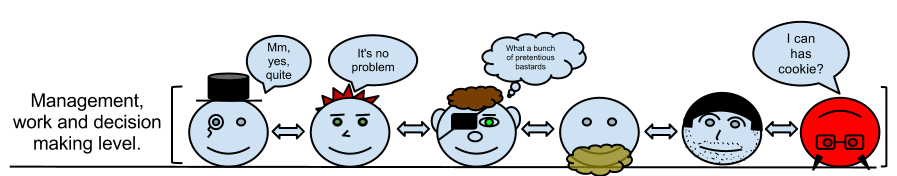
\includegraphics[width=\textwidth]{TeamOrganizationchart}
        \caption{Team Organization chart}
        It was made during lunch, but the general principle still remains, that the structure is flat.
        \label{fig:TeamOrganizationchart}
    \end{figure}
    
    %Why changing roles does not work in our structure and how we solve the challenges that might occur in this association. 
    As the structure shows in the chart, there is no difference in what responsibility level anyone have, or what role one has. The concept of changing roles weekly is good for a learning situation, but very inefficient where knowledge and research are key components in a limited timed project. We anticipate that the time for this project probably won't be sufficient for any role changes, and therefore we have to keep people focused on the task they have been assigned. The efficiency of the current task relies on having the current research fresh in mind. If we were to change the roles every week, the newly assigned person would spend much time getting up to date at the beginning of every week, which in turn wouldn't yield any measurable gains. 
    
    Rather than focus on responsibilities within the group, we've chosen to focus on tasks.
The task will to some degree still represent areas of responibilities, and since tasks will be spread across several group members, we don't run the risk of  a single missing member crippling the entire group. Instead the remaining member$($assigned$)$ to a task will be able to pick of the slack. This, together with thorough documentation of a members knowledge, will just about eliminate the problems associated with an absent group member.
        
    Further, the team structure and the distribution of responsibility gives us the chance to define how we want to deal with task and their priority. The work flow that we have makes us prioritise tasks continuously and get the most pressing task done at the correct time. It's similar to a max heap. We put tasks in to the heap, heapify(prioritise tasks) and choose(pop) the maximized task, the task that has the highest priority. 
    
    %Task division and delegation.
    When we choose a task we consider the person's interest, experience and existing knowledge. Most times the tasks fall naturally to one person that has worked with similar tasks earlier in the project. Other times there is more of lottery, where the task has no prerequisites. Often we rely on a person's initiative to take a task or we easily delegate them with a question, "Can someone do that?". Task delegation and sharing the work load has not been a problem so far in the project.
    
    %benefits of a flat team structure. Not very important. 
    
    \subsubsection{Team communication}\label{Team communication}
    We decided that we will work together from 10 to 16, Monday through Thursday every week, with allowed exceptions for lectures and such. Group members can also work in their free time to make up for missed collaboration hours or to just put in some extra work. This means more work than the course requires, but we decided that we want to do it this way so we can either take some time off now and then, or have more time for the exams in May.

    We will not be able to have frequent face to face meetings with the customer, but we will have weekly online meetings with them instead, as well as e-mail communication as needed. Since we have seen what happens in projects where there is little to no communication, we decided, in agreement with the costumer, that we at least wanted to have weekly meetings in order to keep a good dialog with the customer, and also give them the opportunity to take part in the development of the project. Because the customer is located in Oslo, we decided that the weekly meetings will be held over Skype.
    
    \subsection{Risk Assesment}\label{Risk Assesment}
    
    \subsection{Process Evaluation}\label{Process Evaluation}
    % Write something about the fact that we use one day a week to work with planning and paperwork. 
    
    Project management documented: 
    Possible deviations and how they have
been handled. 

    \subsection{Progress tracking and Documentation}\label{Progress tracking and Documentation}
    In the beginning we had a summary every day where we wrote what we were working on and what had to be done. We stopped doing this after we got good activity plans because the daily summaries became unnecessary. 
    
    \begin{figure}[h]
        \centering
        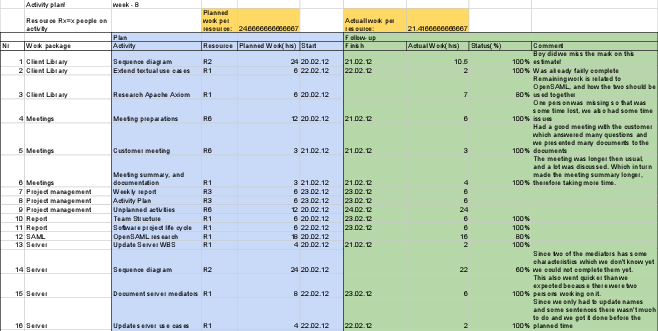
\includegraphics[width=\textwidth]{Week8activityplan}
        \caption{Example Activity plan}
        \label{fig:Week8activityplan}
    \end{figure}
    
    The activity plans(Fig:\ref{fig:Week8activityplan}) now have the role of our day to day summaries and work progress. We update the activity plan as we go along. This way we have a complete overview of tasks and work hours that are planned this week. As we update the activity plan we have an overview of the work done this week and where we have missed with our time estimation. 
    
    \begin{figure}[h]
        \centering
        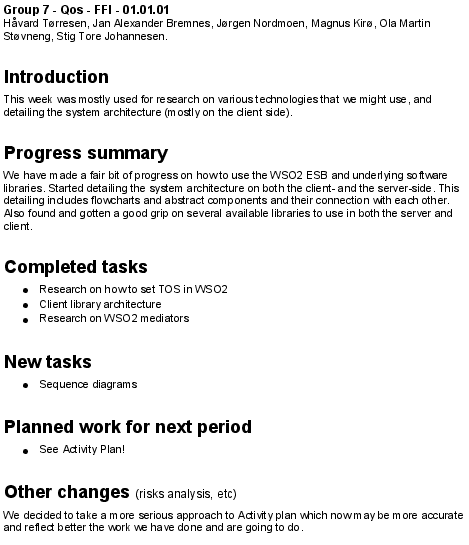
\includegraphics[scale=0.5]{Week7statusreport}
        \caption{Status report example}
        \label{fig:Week7statusreport}
    \end{figure}
    
    As we can se in the weekly report (Fig:\ref{fig:Week7statusreport}) the staus report ha a standard setup. We created a template early in the project so that we did not have to redo the work later. In the prosess of creating the template we put some thought in to it so that we would get a template that would work throughout the project without further changes. 
    
    % write description    

    
    The activity plan has a template which we clone every week to create the plan for next week. We update it  







\section{Development Methodology}\label{Development Methodology} 
    We did not follow any established development methodology, such as \gls{scrum}\footnote{\gls{scrum} - An agile software development methodology. [\url{http://en.wikipedia.org/wiki/Scrum_(development)}]} or \gls{xp}\footnote{\gls{xp} - A type of agile software development. [\url{http://en.wikipedia.org/wiki/Extreme_programming_practices}]}, as this project required more planning and configuration of existing solutions, than actual coding. In the process of choosing a development methodology we considered scrum, waterfall, agile, xp, and some others in addition to combination of these. In the end we chose a mix of the \gls{waterfall}\footnote{\gls{waterfall} - A sequential design process. [\url{http://en.wikipedia.org/wiki/Waterfall_development}]} and \gls{agile}\footnote{\gls{agile} - A group of software development methodologies based on iterative and incremental development. [\url{http://en.wikipedia.org/wiki/Agile_software_development}]}, we discuss these decisions in the sections below. You will also 
find a list of the tools we chose to work with, and why we decided to use them. 
    
    Because this was a research project, the customer would act more as an advisor than a customer, and would have more suggestions and advice than demands and requirements. We had been given a clear understanding of what the final product should be, and we had a list of requirements that would be met. Other than that, we were relatively free regarding how we go about solving the problem. Because of this, a single methodology, like Scrum, wouldn't work for us, as it would require us to be in close and frequent contact with the customer, presenting a prototype at regular intervals, and continue development based on the customers feedback and demands.
    
    As mentioned, this was a project that required quite a lot of planning before any programming could be done. This necessitated that we started the development according to a waterfall model in terms of the architecture planning, as well as the requirements specification. By using the waterfall model in these first phases, we ensured that the planning was done thoroughly in order to minimize the amount of trial and error during the later implementation phase.
    
    As the project progressed we switched to a more agile development method, in order to allow iterative development and facilitate necessary changes that have turned up as code was produced, as opposed to waterfall-coding, where we would have to strictly follow our plans. Agile also let us use the flat organizational structure we had chosen, which we believed would greatly help cooperation within the team.
    
    \subsection{Project Organization}\label{Project Organization}
    
    We divided the project tasks into work packages. These packages are represented in a \gls{wbs}\footnote{\gls{wbs} - An oriented decomposition of a project into smaller components. [\url{http://en.wikipedia.org/wiki/Work_breakdown_structure}]} (ref:~\ref{Work Breakdown Structure}). The schedule for the project is represented in a \gls{gantt}\footnote{\gls{gantt} - A type of bar chart that illustrates a project schedule. [\url{http://en.wikipedia.org/wiki/Gantt}]} (Fig:~\ref{fig:gantt}). The figure is part of our full Gantt chart. As the full diagram cannot be included nicely in the report we have attached it as an HTML document (ref:~\ref{File Attachments}).
     
        \begin{figure}[h]
            \centering
            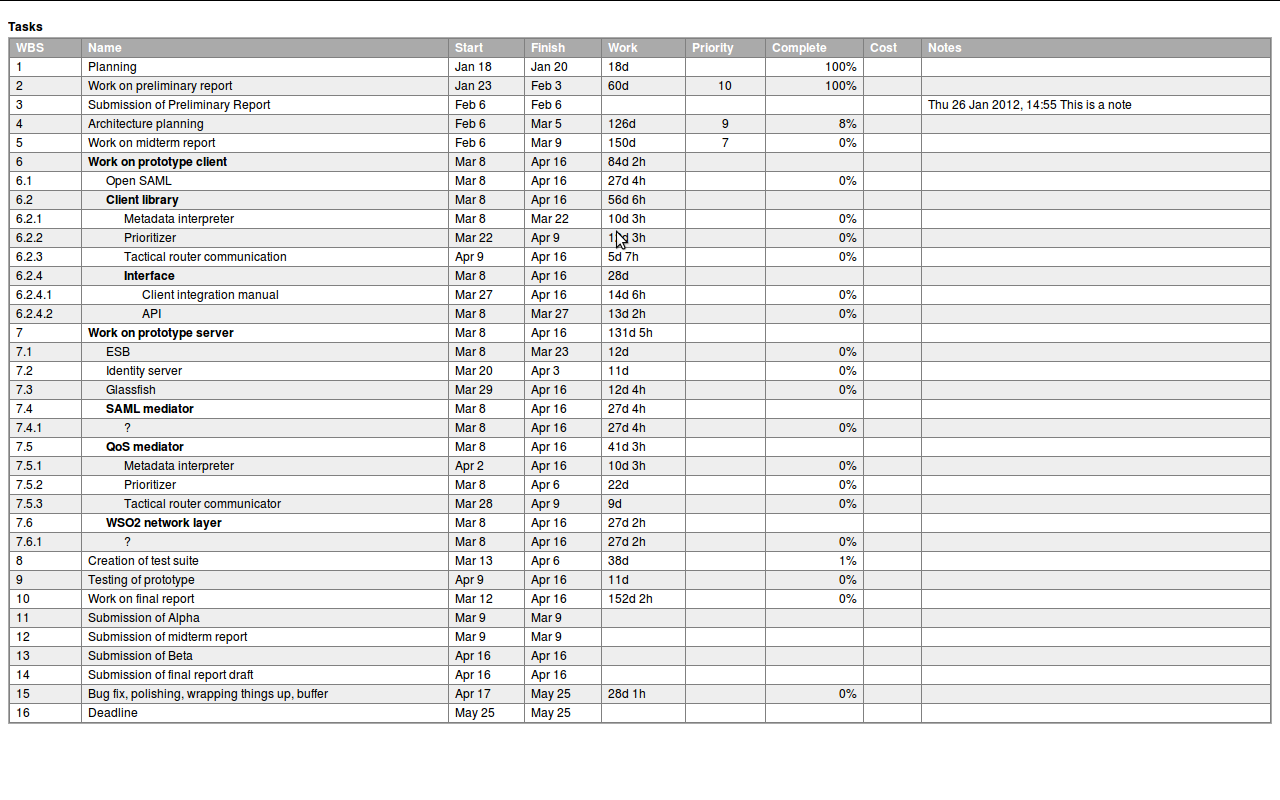
\includegraphics[width=\textwidth]{gantt}
            \caption{Part of our Gantt diagram} 
            This is an example to show that the gantt diagram exists and what it looks like. Se full diagram under file attachments (ref:~\ref{File Attachments}).
            \label{fig:gantt}
        \end{figure}
    
    \subsection{Software project life cycle}\label{Software project life cycle}
    
    For our project life cycle we chose agile. Originally we started out with the intention of using Scrum and Scrum only. That idea was quickly scrapped as we found out that our task was very research heavy. This made us rethink our approach to the development cycle and turn in the direction of agile software development.
    
    Early in the project we expected that we could begin coding and prototyping before too long. This proved to be wrong as there was a lot of research to be done. Scrum was originally a tactic to improve product flexibility and production speed. This works very well in software development when you already know what you are supposed to do and the major part of the task is to implement the required functionality. When the functionality has to be designed and researched extensively, scrum becomes unsuitable. 
    
    With the agile method there are elements that suits us better than others. "Individuals and Interaction" and "Customer Collaboration" are two important elements that we use. The full description of the agile method can be found in the Agile Manifesto\footnote
        {Agile Manifesto, the key elements of the agile software development method. [\href{http://http://agilemanifesto.org/}{AgileManifesto.org}]}.
    
    "Individuals and interactions" is strongly connected with the organization of our team (ref:~\ref{Team Organization}). The flat team structure forced us to have a good dialog among the group members. This increased the team members' interaction and strengthens the team communication. The strengthened communication promotes the individuals of the group and the team members' confidence, which in turn increases the total productivity of the group. The frequent interactions with the customer are also a part of our adaption to the agile development method. 
    
    "Customer Collaboration" is the aspect of the group contacting the customer and keeping a good dialog with them. This was to make sure that we produced the product that the customer wanted. To achieve this part of the agile manifesto we had meetings with the customer every week, and had frequent email correspondence to iron out the bumps in our product. The frequent communication with the customer helped us to create a more precise and consistent system with better documentation. The main part of the communication with the customer was for the benefit of the project, and constant improvement. The constant improvement and iterative work flow is a central part of the agile method. 
    
    Scrum is an agile development methodology. Waterfall is not. Waterfall takes development very much a step at a time. While agile-like approaches like scrum run around a track, repeating its steps over and over. The common steps of waterfall and scrum agile are: planning, build, test, review, deploy. 
               
    Scrum does these steps in an iterative manner. First planning, building, testing and then review. These steps are repeated several times before another bigger review is done, followed by testing. This cycle repeats over and over, until the project is done. 
    
    Waterfall  does these steps one at a time. First the planning part until all the planning is complete. Then the implementation part where all the coding is done. Testing follows as a natural step. The testing is thorough, so that no more coding or testing has to be done. Then the review part follows, where functionality, requirements and completeness is assessed. And deployment comes as the last step, when everything is working as it should and everything else is complete.  
    
    We ended up using something like iterative waterfall. Where we planned a lot in the beginning, started coding and testing nearly at the same time, the testing consisting of unit tests at that stage. While coding we had reviews and a bit of quality control of the code. When the code was complete we started system testing. System testing and code improvement went in iterations as we found problems and mistakes that were overlooked before. Then we followed with the documentation part, representing a sort of deployment phase of the waterfall methodology. 

    \subsection{System Technology}\label{System Technology}
    
    To begin with we intended to use \gls{junit}\footnote{\gls{junit} - A testing framework for the Java programming language. [\url{http://junit.org/}]} tests throughout the project. This started well in the implementation phase, but faded away towards the end of the implementation phase; especially when the implementation was a week delayed and we used a lot of time debugging and making the system actually work. 
    
    At the beginning we planned to have code reviews and go through all the code and fix code deficiencies. This was meant to happen every other week. As good as this intention is we didn't manage to do it as often as we would like. In the server side we had two code reviews. With the client we had none. We also experienced that the code reviews didn't really work out as we had planned. While debugging the client library and the server side of the developed application we found a lot of bugs and logic errors after the code reviews. This means that our code reviews were bad and that they didn't really fulfil their purpose. 
    
    One of our requirements was that the system should be thoroughly tested. To accomplish this requirement we decided to use the MobiEmu framework. MobiEmu is a network emulator that emulates network traffic and behaviour. It is based on NS3 and can test multiple nodes in a virtual network. This gives us the advantage of testing our system to a good extent of the real time battle situation that the system is thought to operate in. Another reason that we used this testing framework is that one of our group members had previous experience with it. The testing framwork gave us useful test results that are discussed in section ~\ref{Testing}.

    Furthermore we used \gls{git}\footnote{\gls{git} - A free and open source, distributed version control system. [\url{http://www.git-scm.com}]} and \gls{github}\footnote{\gls{github} - A web-based hosting service for software development projects that use the Git version control system. [\url{http://www.github.com}]} to handle our files and repository. 
    
    Along with git we used Google-docs, now drive, to store and share documents. This helped us greatly in the cooperation of this project. Google docs allowed us to be multiple people to working on the same document at the same time. 
    
    \gls{latex}\footnote{\gls{latex} - A document preparation system for the \TeX -typesetting program} is obviously the preferred report scripting language for the task of writing this report. Latex helped us a lot in the report writing process. Syntax highlighting, easy integration of figures and good structure to the report files are examples of benefits we got from using \Tex.
    
    With input from the customer and their approval we decided to use Apache2 license for our code. As far as all parties could find, there was no negative side for any of us. 

    As for the personal development environment, the individual person was responsible to get his system to work. While the choice of environment is free we presume that we achieved greater productivity than if everyone were forced to use the same environment, e.g: ubuntu with eclipse.  

    As for a total list of tools that was use, see the section about Tested tools, (ref:~\ref{toolslist})    
    

\section{Prestudy}\label{Prestudy} 
	This project was one that requires quite a lot of prestudy before we could begin coding or even designing the architecture. Since the customer wanted us to implement existing technologies, such as Glassfish, WSO2 and SAML. We needed to spend some time researching those technologies to figure out what to use, and how to use it. The following sections  describes the the overall architecture of how we imagined our system to be like. 

        \begin{figure}[htb]
            \centering
            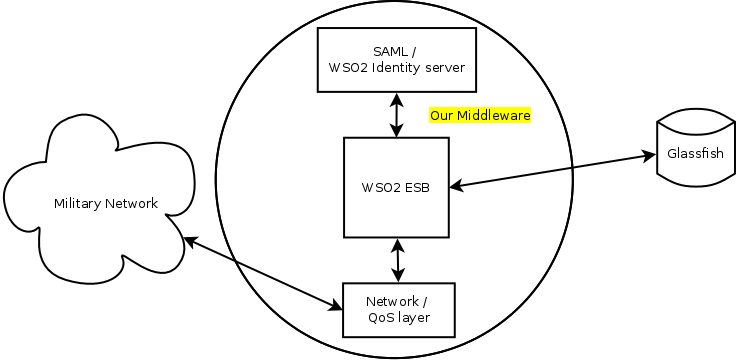
\includegraphics[width=\textwidth]{birdarch}
            \caption{Basic server architecture}
            This shows our initial thoughts of how the servers side architecture would look like. This was changed later in the project. 
            \label{fig:birdarch}
        \end{figure}

    \subsection{Server side Architecture}\label{Server side Architecture}
        The server side architecture consists of several components, the WSO2 ESB, the \gls{tr} and the GlassFish server. Most of them are visible in the initial architecture shown in Fig:~\ref{fig:birdarch}. All of these components are already available, so what we needed to make were \glspl{mediator}\footnote{\Gls{mediator} - A component in WSO2 ESB which can be used to work on incoming or outgoing messages that passes through the ESB} in the ESB.


        Before the client can request a Web service it has to have an identification. To get an ID-\gls{token} it has to contact the Identity Server using the ESB as a \gls{proxy}\footnote{\Gls{proxy} - A proxy server acts as an intermediary between clients and servers} (Fig:~\ref{fig:Serversidearchitecture}-1). Then the client can request a Web service from the ESB. Several things will then happen in the ESB. First the request message is sent to the SAML mediator (Fig:~\ref{fig:Serversidearchitecture}-2), this mediator contacts the Identity Server to validate the clients ID-token (Fig:~\ref{fig:Serversidearchitecture}-3). If the token is validated and the client is supposed to have access to the requested service, the message is passed on to the GlassFish proxies (Fig:~\ref{fig:Serversidearchitecture}-4), otherwise it is dropped. The ESB acting as a proxy will then send the request along to the requested service on the GlassFish server (Fig:~\ref{fig:Serversidearchitecture}-5).

        \begin{figure}[htb]
            \centering
            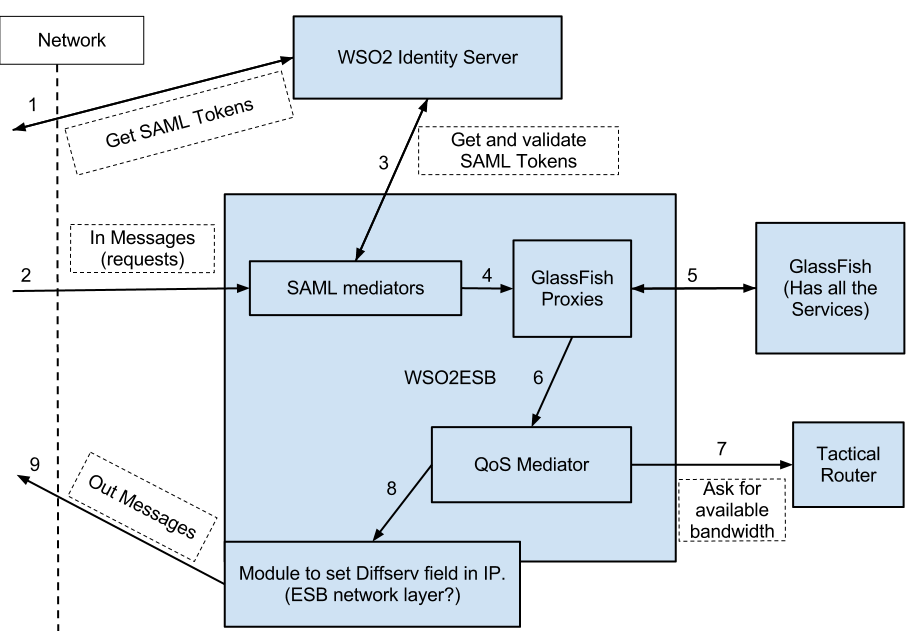
\includegraphics[width=\textwidth]{Serversidearchitecture}
            \caption{The Server side Architecture}
            This is the overall design of our implementation of the server side. It shows the modules in the server and the flow in the system. 
            \label{fig:Serversidearchitecture}
        \end{figure}

        When the request is received at the service, it will probably start sending some data to the client. This is also done through the ESB. First the message is sent to the QoS mediator (Fig:~\ref{fig:Serversidearchitecture}-6). This mediator will first look at the role, or identity, of the client and the service requested, and use this information to assign a priority to the connection. Then the \gls{monitoring service}\footnote{Monitoring Service, a service that provides bandwidth monitoring, running on the same server as the \gls{tr}}(from here referred to as \gls{ms}) on the \gls{tr} is contacted for bandwidth information (Fig:~\ref{fig:Serversidearchitecture}-7), which is used together with the priority to determine whether the message should be sent right away or held back until some higher priority message is finished sending.

        Either in the QoS mediator, in the ESB’s network layer, or after that, the DiffServ (ToS) field of the IP header will have to be set (Fig:~\ref{fig:Serversidearchitecture}-8) before the message is sent to the client (Fig:~\ref{fig:Serversidearchitecture}-9). This field is used by the routers in the network to prioritize packet sending. This step is quite important to the whole procedure as this is one of the few requirements the customer has given us. As such this step can not be dropped from the final product.

 
    \subsection{Client side Architecture}\label{Client side Architecture} 
    
        The client-side architecture will be composed of altered (already existing) client software, the \gls{opensaml}\footnote{\gls{opensaml} - A set of open source C++ and Java libraries to support developers working with SAML. [\url{https://wiki.shibboleth.net/confluence/display/OpenSAML/Home/}]} library as well as our client library implementation.
        
        \begin{figure}[htb]
            \centering
            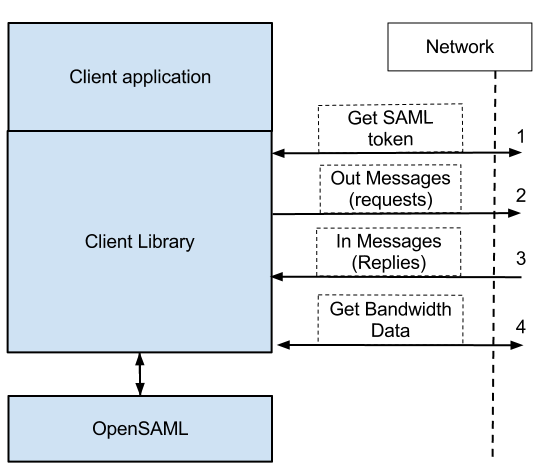
\includegraphics[scale=0.5]{Client-sideArchitechture}
            % do not import the new figure as the old one is corret as this is the prestudy. 
            \caption{The Client side Architecture}
            The client architecture shows the basic thought of what the system should look like and the communication to and from the client library. 
            \label{fig:Client-sideArchitechture}
        \end{figure}
 
        Before the client library can ask for the data the client needs to get a SAML authentication token from the identity server (Fig:~\ref{fig:Client-sideArchitechture}-1). The communication here will most likely be handled by our library, but the SAML packages will be created and analyzed by the OpenSAML library. 

        The client library then sends the request from the client to the server (Fig:~\ref{fig:Client-sideArchitechture}-2), appending the SAML token to the package as well as adding some metadata in the SOAP header related to the client role and setting the TOS field of the package to a default value.

        The reply from the server is examined by our client library for the metadata the server has embedded in the SOAP header. Relevant metadata is stored for future communication and the package is passed to the client application (Fig:~\ref{fig:Client-sideArchitechture}-3).


        When new communication is initiated after this first connection is made the client should, if everything went as expected, have the necessary information to prioritize new messages. This means that the client can now take an informed decision about how it should prioritize messages, but in order to do this to the best of it's abilities it also has to take into consideration available bandwidth (Fig:~\ref{fig:Client-sideArchitechture}-4).
    
    \subsection{Unit testing}\label{Unit testing}
    We decided quite early on that we wanted to do unit testing of every piece of code that we would produce, i.e., test driven development. The reason behind this choice is that we think it will result in better code quality. An added bonus is the simplification of integration testing, due to easier discovery of whether a new code addition will integrate with the old code. Also writing the tests first lets us concentrate more on exactly what the methods should do, instead of the content and how it should do it. One of the problems with test driven development however, is the possible bias that could occur, we could end up only satisfying the test and not the actual requirements. This could be countered to some extent by writing more comprehensive tests. Another positive point in favour of unit testing is the requirement we have, which states that the product has to be written in Java where such test are easy to integrate and write using JUnit.

    \subsection{Integration testing}\label{Integration testing}
   For integration testing, we decided that we wanted to do automated system testing every other week in collaboration with code reviews. The procedure we are going to follow will be coding new features in a separate branch. Once every other week the finished branches will have all their unit tests run thoroughly, followed by a code review of at least one person. Then if the automated system tests are fully operational, they will also be run to look for additional errors which the unit tests cannot pick up. This point is likely to change in the future as a two week time interval might be too long given the short implementation period. The advantage of doing this integration testing is better overall code quality, since we test code before it is used by other parts of the system. Since we are also doing code reviews, people will also gain experience with other parts of the system which they previously had not worked on. This will benefit everyone since knowledge about the system is shared, and it will 
help in the eventuality of someone getting sick. The advantage of developing in separate branches is the reduced risk of polluting code other people are working on, and a better separation of stable and unstable code.

    \subsection{System testing}\label{System testing}
    
    When it comes to system testing, the customer was quite insistent that we test the product thoroughly in an emulated network situation. Since we have had some experience with ns-3\footnote{ns-3 is a discrete-event network simulator for Internet systems, targeted primarily for research and educational use. - [\url{www.nsnam.org}]} we decided that we wanted to do the system testing on it. Following we describe the initial advantages of the testing freamework and test cases we were going to use. 
    
    The advantage with this, is that the customer has already set up some testing scenarios and helper-scripts designed for ns-3, which they offered for our use. This will greatly reduce the time needed for setting up the test suite, and it will also give us the ability to have automated tests, which we don’t have to monitor or interact with.
    
     Another added advantage is easy testing, as we only have to start a script in order to run the whole suite, but that comes at the cost of actually setting up the whole thing. As of the midterm report, we have set quite a lot of time aside in order for us to implement the proper ns-3 support we need. 
        
    To monitor what is happening during the test-runs, our applications will output all important information regarding what is going on, in addition to this we have a \gls{packet sniffer} on each end which will capture network traffic. Using this information we should be able to tell a whole lot about what is going on in the network and we should be able to decide whether we have met the requirements or not.

    Below are some of the detailed test cases which we want to automate on top of ns-3. The testing itself will be automated, but in order to get some result from the tests, some human interaction is needed to interpret the output data.
\\
    \begin{figure}[h]
        \centering
        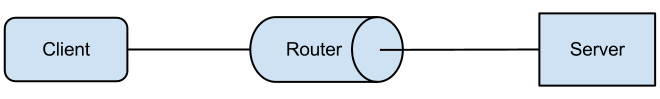
\includegraphics[scale=0.4]{Simplemessagesending}
        \caption{Simple message sending}
        One client communicates with one server through one router.
        \label{fig:Simple message sending}
    \end{figure}
\\
Simple message sending:\\
    In this test, shown in Fig:~\ref{fig:Simple message sending}, we want to test the ability of the client and the ESB to communicate. We want to see that the client is able to send messages (definition can be found in the glossary under "\gls{message}") to the server and get a response back. For monitoring purposes, this test will rely on both applications to log their behavior. In order for us to give this test the green light we must see a message going out from the client then passing through the ESB to GlassFish. Then finally a reply should be sent back from GlassFish to the ESB and then to the client.

\\\\
Setting Quality of Service:\\
    In this test, we want to test the client and the ESB’s ability to set the DiffServ field in the IP header. The first requirement is that the test “Simple message sending” has been passed. For this test to be considered a success, the client has to send a message to the ESB, which responds with the DiffServ value in the SOAP header. The ESB must at this point have set the DiffServ value in the IP header. The client should then use a service on GlassFish, but this time the IP header must contain the correct DiffServ value. In order to monitor this test, only a packet sniffer located on the client and ESB side needs to be used. The packets must be examined, and the correct DiffServ value must be present in the IP header of all packets, except the first one going out from the client.
\\
    \begin{figure}[h]
        \centering
        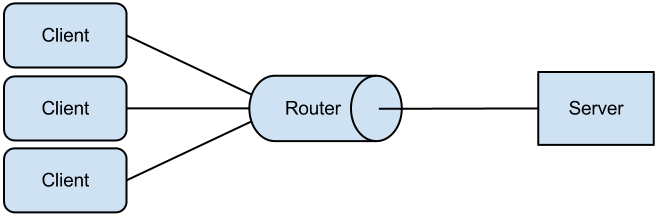
\includegraphics[scale=0.4]{3Clientmessagesending}
        \caption{Three clients message sending}
	Three clients communicate with the same server through the same router. One of the clients will have a higher priority than the two others, in order to test the servers ability to prioritize.
        \label{fig:threeclientmessagesending}
    \end{figure}
\\   
Prioritizing messages:\\
    In this test we want to test the ESB’s ability to prioritize messages. The scenario will be set up as shown in Fig:~\ref{fig:threeclientmessagesending}, with two clients sending lots of messages in an attempt to flood the capacity of the network. All of these messages should have the same priority, but intermittently, a third client with a higher priority will attempt to send some messages. What we are looking for is that these higher priority messages should be sent out from the ESB before the ones with lower priority and, if necessary, it has to stop some already being sent messages. For this test to be successful, we must see some lower priority messages being preempted or held back. To do this, the log file of the ESB must be studied, and there should be some clear indications of one of the requirements.
\\\\
Changing DiffServ value:\\
    In this test we want to check the ESB’s ability to change the DiffServ value after a reconfiguration. The test can be performed and the result examined the same way as “Setting Quality of Service”, but this time the test has to be run twice. One where the configuration has one DiffServ value, and a second run where the DiffServ field has a different value. For the test to be successful, one would have to examine the resulting \gls{pcap}\footnote{\Gls{pcap} is short for Packet capture, which in our text usually refers to a program which captures the traffic on a given socket} files on the server side, and check each run to see if the two tries have different DiffServ values.
\\
    \begin{figure}[h]
        \centering
        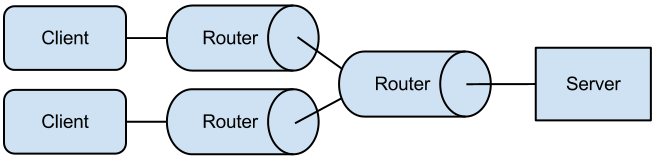
\includegraphics[scale=0.4]{2Clientdifferentpathsmessagesending}
        \caption{Two Clients with different paths}
        Two  clients communicating with the same server, but with different paths.
        \label{fig:2 Clients different paths message sending}
    \end{figure}
\\    
Multipath server routing:\\
    In this test we want to look at the ESB’s capabilities to talk to the MS and understand the routing result. From the MS the ESB should get some routing information about the topology of the network. As you can see in Fig:~\ref{fig:2 Clients different paths message sending}, if the link between the server and the first router is not the limiting factor, the two clients should not get in each others way. Therefore, since we get the information about the last router from the MS, the ESB should understand that there is likely no problem and should not preempt any messages. To check if this is actually the case, the ESB will need some time to adjust as it does not get the full picture of the network topology, but after this time, no messages should be dropped from the ESB’s side.
\\
    \begin{figure}[h]
        \centering
        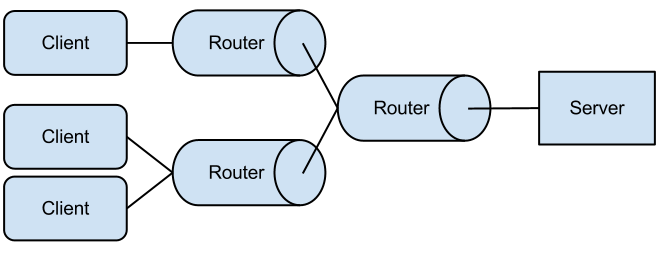
\includegraphics[scale=0.4]{3Clientswheretwoarecompeting}
        \caption{Three Clients where two are competing}
        Three clients communicate with the same server, but only two of them share the path.
        \label{fig:3clientstwocompeting}
    \end{figure}
\\
Competing clients in a multipath environment:\\
    This test is a compilation of the tests “Multipath server routing” and “Prioritizing messages”. For this test we want to make sure that the ESB is smart enough to only preempt the messages going to one of the competing clients. As you can see in Fig:~\ref{fig:3clientstwocompeting}, there is one client which should not affect either of the two others if the link between the server and the first router is not a bottleneck. This should allow this client to receive messages even though the two other clients are competing for scarce resources. To check that this test is successful, a combination of the client's log files and the server log files will have to be used. If most (over 96\%) of the messages arrive at the higher priority client and the third client is not affected then this test is successful.
\\\\
Competing clients in a low bandwidth scenario:\\
    In this test we want to test that the ESB can manage to prioritize messages in a network with a joint bottleneck, but with different endpoints. In Fig:~\ref{fig:3clientstwocompeting}, if the link between the server and the first router is the bottleneck, the ESB should, after a small initialization period, understand that it has to preempt messages going out to all clients, in order to let a higher priority client get the service it is supposed to get. The scenario will be set up in such a way that one of the two competing clients will have higher priority than the two others, the two lower priority clients should then send a steady stream of messages, which should fill the bottleneck link. The third client should then start sending some messages which must now fill the entire bottleneck link, and create a situation where the ESB has to hold back or preempt messages going to either of the two other clients. As before, a combination of the ESB and the client's log files have to be examined.
           
    \subsection{Alternative solutions}\label{Alternative solutions}
        The customer also gave us a paper\cite{soa-qos-pdf} which described a previous project they had worked on which tried to solve something quite similar to what we were tasked with. The paper described a system which were used in conjunction with \gls{tr}s to retrieve bandwidth information and to control transmission of messages into this network. As the customer explained this work was not something we could directly copy as the project had not used a lot of web standards and had focused more on the \gls{tr}s as opposed to Web services. What we could take out of it however was how they throttled messages. The paper contained five methods which we could easily implement and use their result as an indication of what methods we should use to throttle or hold back messages.

        One architecture, which our customer suggested for the project, was to have a proxy in between nodes and creating a custom QoS layer which would sit in front of both the client and the services. This layout can be seen in Fig:\ref{fig:alternativesolution}. This layer would then communicate with a SAML server for authentication, and would have to do all the message prioritization based on the same criteria as our architecture. There are several points about this architecture which would make it a good fit for us. Since the QoS layer would be identical on both client and server side it would mean less work, and more code that could be shared among components, but this freedom comes with some downsides. The first and most glaring problem encountered would be that services on the server would have to be altered to be able to communicate with this front end. Even though we were free to choose architecture ourselves, the client expressed a wish that we would not choose this model because the customer wants 
to use \gls{cots}\footnote{\gls{cots} - Commercially 
available Off-The-Shelf} services which would not be compatible with the new front end.

		\begin{figure}[H]
			\centering
			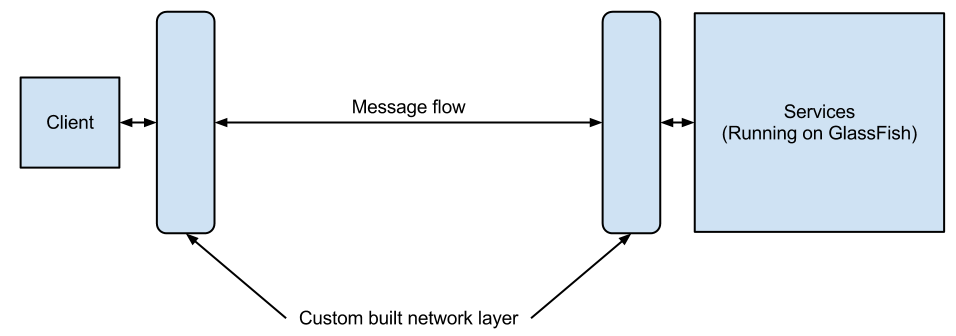
\includegraphics[width=\textwidth]{AlternativeSolutionadaptservicesandclients}
			\caption{Alternative solution}
		Alternative solution where both clients and services are adapted with a custom layer.
			\label{fig:alternativesolution}
		\end{figure}

        Even though the above-mentioned architecture is not the best fit for us we wanted to take some aspects of the architecture further. Since clients can easily be altered, the above mentioned solution is not applicable for server side, the solution could however be used for the clients. Having a proxy on the client side could be quite good, but because of the work involved and probable time constraints we chose not to go with this solution. On the server side however a front end is not the best solution for us. What we instead are looking into, is to use an ESB which would be configured together with the services and work as a proxy. Because many ESBs have integrated SAML processing we could easily take advantage of such facilities along with custom message processing, with which we would then extend the ESB to support our needs. The clients would have to point to the ESB, but this should both be trivial to do and the customer has expressed their agreement that this is satisfactory. We could eventually 
expand the functionality with service discovery, which then would be a good solution to the problem.

        So far we have outlined major alternative architectures which could be alternatives to our project, but there are also alternatives within our proposed solution. One such alternative is not to use a premade ESB, but rather build one ourselves. This solution was thoroughly investigated, but was eventually turned down because of the massive amount of work that would involve, the quality of an already made ESB is much higher than we could ever achieve during this project, and lastly, the open source tools available to implement the functionality needed for SAML was not very well documented, and would take considerable time to get familiar with.
        
        \begin{figure}[H]
			\centering
			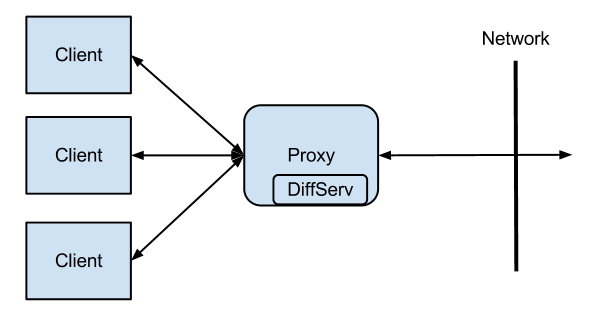
\includegraphics[scale=0.4]{Clientswithproxy}
			\caption{Alternative solution with proxy}
		Alternative solution where clients contact a HTTP proxy to communicate with services.
			\label{fig:alternativesolutionproxy}
		\end{figure}

        On the client side we also have the choice of having either a \gls{http}\footnote{Hypertext Transfer Protocol} proxy or writing our own custom library. Both have some advantages and disadvantages, a proxy would be better for integration with client programs, but creating this proxy or configuring and customizing an already existing solution is not trivial. An outline to this solution is seen in Fig:\ref{fig:alternativesolutionproxy}. On the same note, creating a library for use in client programs is easier, but this would mean that client programs would need to be altered to be usable with our middleware, which isn’t particularly desirable. We chose to go down the road of least resistance, as we see it currently we would have do quite a lot of research into proxies which could in the worst case scenario result in just wasted time as far as our product goes. A client library would from our perspective be easier as we would have more control, the overall design should be easier and we know that with 
this sort of library we can integrate OpenSAML which is a huge advantage.  
    
    \subsection{Process model}\label{Process model}
    Before we started this project we were quite unsure how we were going to work on the project. We had heard lots about Scrum, but few of us had ever used it in a project of this scale. For us this meant that we had lots of options, but we did not know a lot about them.
    
    After we talked to the customer about what the task was, and understood what we were going to do, we decided that we wanted to use a Waterfall model\footnote{\gls{waterfall} - A sequential design process. [\url{http://en.wikipedia.org/wiki/Waterfall_development}]}} of software development. Because our assignment is quite research-focused we need to start with a planning stage in order to completely comprehend the task ahead and how we are going to solve it. This method of working lends itself very well to the Waterfall model, but we feel that it would not work so great with Scrum or a more agile method. This does not make Scrum completely impossible, but it would be harder than the Waterfall model with little extra reward. Our choice of process model is described in section~\ref{Software project life cycle}.
    
    To practice some agile development we decided that we want to make the implementation phase as agile as possible. This would mean weekly sprints with code review and rapid delivery. This would be something that we could do after the planning phase is done to hopefully produce higher quality code. The reason behind this decision was our interest in Scrum or agile development and the thought that weekly sprints with code review will improve the overall code quality and help us keep our eyes on the prize.
    
    \subsection{Tools}\label{Tools}    
    We had no clear outline of what tools we were going to use in the prestudy phase. The tools we ended up using are described in \textit{System Technology~\ref{System Technology}}.
          

\section{Design}\label{Design}
    \subsection{Client Side}\label{client side}

This chapter will introduce the design and architecture of the client side of our system. Section \ref{client introduction} will introduce the different components that make up the entire client, and includes a description of the different components that make up the client library. Next, section \ref{client use cases} will describe the use cases, and section \ref{textual client data flow} will take care of the data flow, followed by a detailed architecture description \ref{client architecture}. Finally, section \ref{client sequence diagrams} will go through the sequence diagrams.
    
    The class diagram is a usefull addition when understanding the architecture of the client library and it's functionality. The descriptions and diagrams in this section might become clearer when looking at the class diagram and see the connections between classes and the more specific contents of the classes. 
		
    \subsubsection{Introduction}\label{client introduction}
The client architecture consists of the following components: The client application, the client library and the Monitoring Service. Additionally, the library makes use of some external components to do some of it's work.

    \subsubsection{Component description:}\label{Component description}

\indent \indent \textbf{Client application:}\\
	The user-controlled applications that utilize web services. These must be modified to send all communication through the client library in order to get the prioritization it should have.
\\\\

\indent \textbf{Client library:}\\
% needs to be rewritten and clearified. 
This component will handle all communication with the service providers, as well as authenticating users and prioritizing their messages, based on who they are, and what their current role is. The authorization will involve a component from the server side of the project, the identity server, which returns a token if the client is authorized. Client applications connect through a simple interface to provide credentials and data.
\\\\ 

    \subsubsection{External libraries:}
\indent \indent \textbf{Axiom:}\\
This component will be used to parse and manipulate \gls{xml}\footnote{\gls{xml} - eXtensible Markup Language} data in the form of SOAP and SAML. These are fairly extensive and complex data structures so an easy to use external library is essential here.
\\\\

\indent \textbf{Apache \gls{httpcomponents}:}\\
A lightweight component for easily setting up and using HTTP connections. While not strictly necessary this component will allow us to connect and communicate across networks far more easily than the standard java componentsy.

	\subsubsection{Use Cases}\label{client use cases}
%%%%%%%%%%%%%%%%%%%%
		\textbf{Title:} Accept client info \\
		\textbf{Actors:} Client software, Client Library Interface \\
		\textbf{Main:}
		\begin{enumerate}
			\item Client software connects to the library interface
			\item Client delivers its credentials
			\item Credentials are passed from the interface to the sequencer.
			\item Credentials are sanitized by the sanity checker and passes.
			\item Credentials are passed from the sequencer to the token manger.
			\item Credentials are stored in the credential store.
			\item Buffer, for previous tokens, is flushed
		\end{enumerate}
		\textbf{Extension:} 
		\begin{itemize}
			  \item[] 4a. Credentials are clearly invalid
			  \item[] 5a. Return error
		\end{itemize}
		\textbf{Precondition:}  None\\
		\textbf{See:} None
		\\\\
%%%%%%%%%%%%%%%%%%%%%%%%%%%%%%%
		\textbf{Title:} Accept data to be sent \\
		\textbf{Actors:} Client software, Client Library Interface \\
		\textbf{Main:}
		\begin{enumerate}
			\item Client delivers data to be sent.
			\item Data is passed to the sequencer.
			\item Sequencer creates DataObject.
		\end{enumerate}
		\textbf{Precondition:} Client has established connection to the Library interface and authenticated it's credentials. \\
		\textbf{See:} Accept client info
		\\\\
%%%%%%%%%%%%%%%%%%%%%%%%%%%%%%%
		\textbf{Title:} Connect to server \\
		\textbf{Actors:} Client Library, Server \\
		\textbf{Main:}
		\begin{enumerate}	
			\item Connection manager connects to the server
			\item Set priority on socket based on SAML-token and related metadata
		\end{enumerate}
		\textbf{Extension:}
		\begin{itemize}
			  \item[] 1a. Unable to connect to server
			  \item[] 2a. Return error
		\end{itemize}
		\textbf{Precondition:} DataObject has been created, and contains both bandwidth info and a token \\
		\textbf{See:} Accept client credentials, Accept data to be sent and Fetch bandwidth info
		\\\\
%%%%%%%%%%%%%%%%%%%%%%%%%%%%%%%
		\textbf{Title:} Get SAML token \\
		\textbf{Actors:} Client library, Server \\
		\textbf{Main:}
		\begin{enumerate}
			\item Client library sends client credentials to server
			\item Server verifies the credentials
			\item Server returns SAML-token
			\item Token is parsed into a token object
			\item Token object is put into DataObject.
		\end{enumerate}
		\textbf{Extension:}
		\begin{itemize}
	        \item[] 2a. Client credentials not valid
			\item[] 3a. Server returns error
			\item[] 4a. Client library throws error
		\end{itemize}
		\textbf{Precondition:} Client has given library credentials and data to send, and a SAML token for the destination doesn’t already exist. Connection to server has been established. \\
		\textbf{See:} Accept client credentials, Accept data to be sent, Fetch bandwidth info and Connect to server
		\\\\
%%%%%%%%%%%%%%%%%%%%%%%%%%%%%%%
		\textbf{Title:} Transaction towards server \\
		\textbf{Actors:} Client lib, server, client \\
		\textbf{Main:}
		\begin{enumerate}
			\item MessageHandler sends buffered data to server
			\item Server returns reply to data.
			\item The ReturnObject in the DataObject gets the data from the server.
			\item MessageHandler send data to sequencer.
			\item Sequencer sends data to interface (QosClient)
			\item Client fires a data received event to all listeners.
		\end{enumerate}
		\textbf{Extension:}
		\begin{itemize}
			 \item[] 2a. Server unavailable, reply doesn’t arrive within timeout, etc.
			 \item[] 3a. Throw error.
		\end{itemize}
		\textbf{Precondition:} Data to send exists, SAML token is in cache, connection to server active.\\
		\textbf{See:} Accept client credentials, Accept data to be sent, Fetch bandwidth info, Connect to server and Get SAML token
%%%%%%%%%%%%%%%%%%%%%%%%%%%%%%%		
		
	\subsubsection{Data Flow}\label{textual client data flow}
        
    \begin{figure}[h]
        \centering
        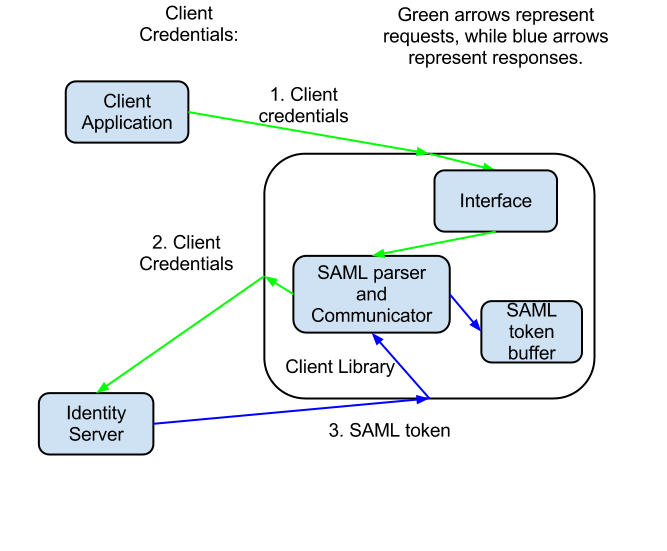
\includegraphics[width=\textwidth]{ClientCredentialsDataFlowDiagram}
        \caption{Client Credentials Flow}
        \label{fig:ClientCredentialsDataFlowDiagram}
    \end{figure}
    
    \begin{figure}[h]
        \centering
        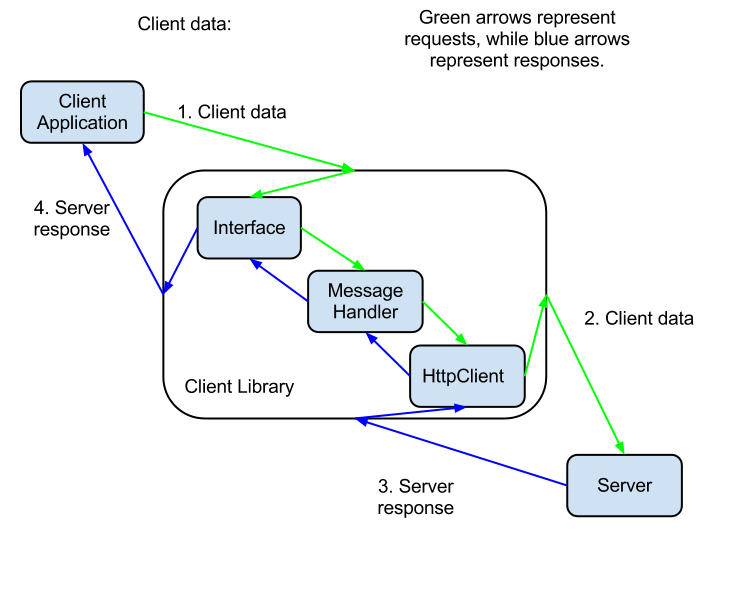
\includegraphics[width=\textwidth]{ClientDataFlowDiagram}
        \caption{Client Data Flow}
        \label{fig:ClientDataFlowDiagram}
    \end{figure}
    
    % the numbering on the figure and in the text does not match. This should maybe be fixed. 
		\textbf{Client credentials} (Visualized in Fig.\ref{fig:ClientCredentialsDataFlowDiagram})
		\begin{enumerate}
			\item From client application
			\item To client library via API/interface
			\item Via SAML to ID-server
			\item Back to client library as valid SAML-token
			\item Stored in library until client App changes credentials
		\end{enumerate}
		
	% The numbering on the figure and in the text does not match. This should maybe be fixed. 
		\textbf{Client Data} (Visualized in Fig.\ref{fig:ClientDataFlowDiagram})
		\begin{enumerate}
			\item Generated by client application
			\item Sent to client library via API/interface
			\item Buffered in library
			\item Sent from library to server
			\item Answer returned to client through library
		\end{enumerate}
		
	\subsubsection{Architecture}\label{client architecture}
		\begin{figure}[h]
			\centering	
			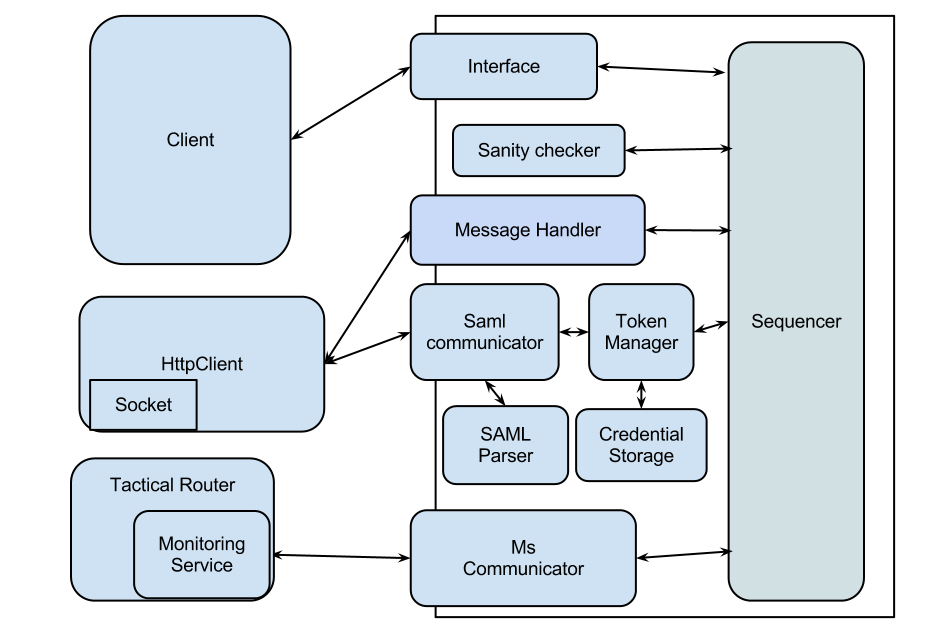
\includegraphics[width=\textwidth]{Detailedclientarchitecture}
			\caption{Detailed Client Architecture}
			\label{fig:DetailedClientArchitecture}
		\end{figure}

    All the following sub paragraphs in this subsection are parts of the client library wich Fig.\ref{fig:DetailedClientArchitecture}.  \\ 
    
		\indent \textbf{Interface} \\
Known in the class diagram as “QosClient”, responsible for providing a clean and easy to use interface for the clients.
\\\\
		\indent \textbf{Sequencer} \\
The central piece of the client library. Responsible for keeping a record of all other modules in the system and communicate between them as well as making sure everything happens in the right order.
\\\\
		\indent \textbf{Sanity checker} \\
	% todo: rewrite this section!
This module is simply there to do some easy verification of data that comes from the client, to make sure that it isn’t faulty in any obvious way (e.g: Data that isn’t xml, or credentials that are empty).
\\\\
		\indent \textbf{Token Manager} \\
This provides a nice and clean interface for the sequencer to store credentials and fetch tokens for data transmissions.
\\\\
		\indent \textbf{Saml Communicator} \\
This module will take care of the communication between the client library and the identity server.
\\\\
		\indent \textbf{Saml Parser} \\
This takes the reply from the identity server and parses it into a token object so that it can be easily used and stored.
\\\\
		\indent \textbf{Credential Storage} \\
Responsible for storing token objects as well as user supplied credentials. Also makes sure that no token objects are returned if they are invalid or expired.

	\subsubsection{Sequence Diagrams}\label{client sequence diagrams}
		\begin{figure}[H]
			\centering	
			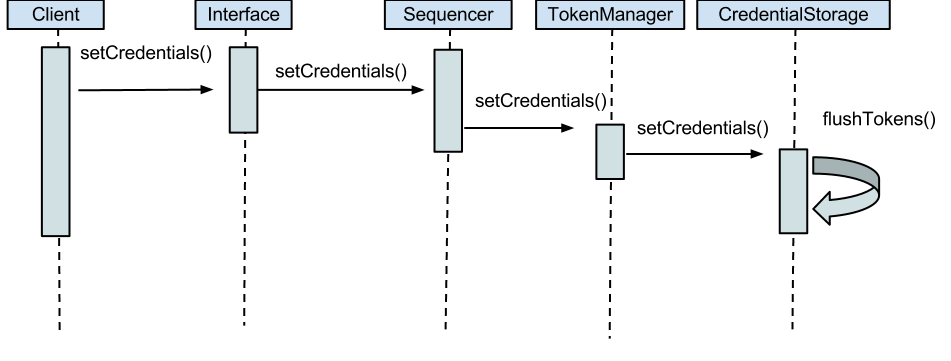
\includegraphics[width=\textwidth]{CliSeqDiaAcceptclientinfo}
			\caption{Accept client info}
			\label{fig:CliSeqDiaAcceptclientinfo}
		\end{figure}
		\begin{figure}[H]
			\centering	
			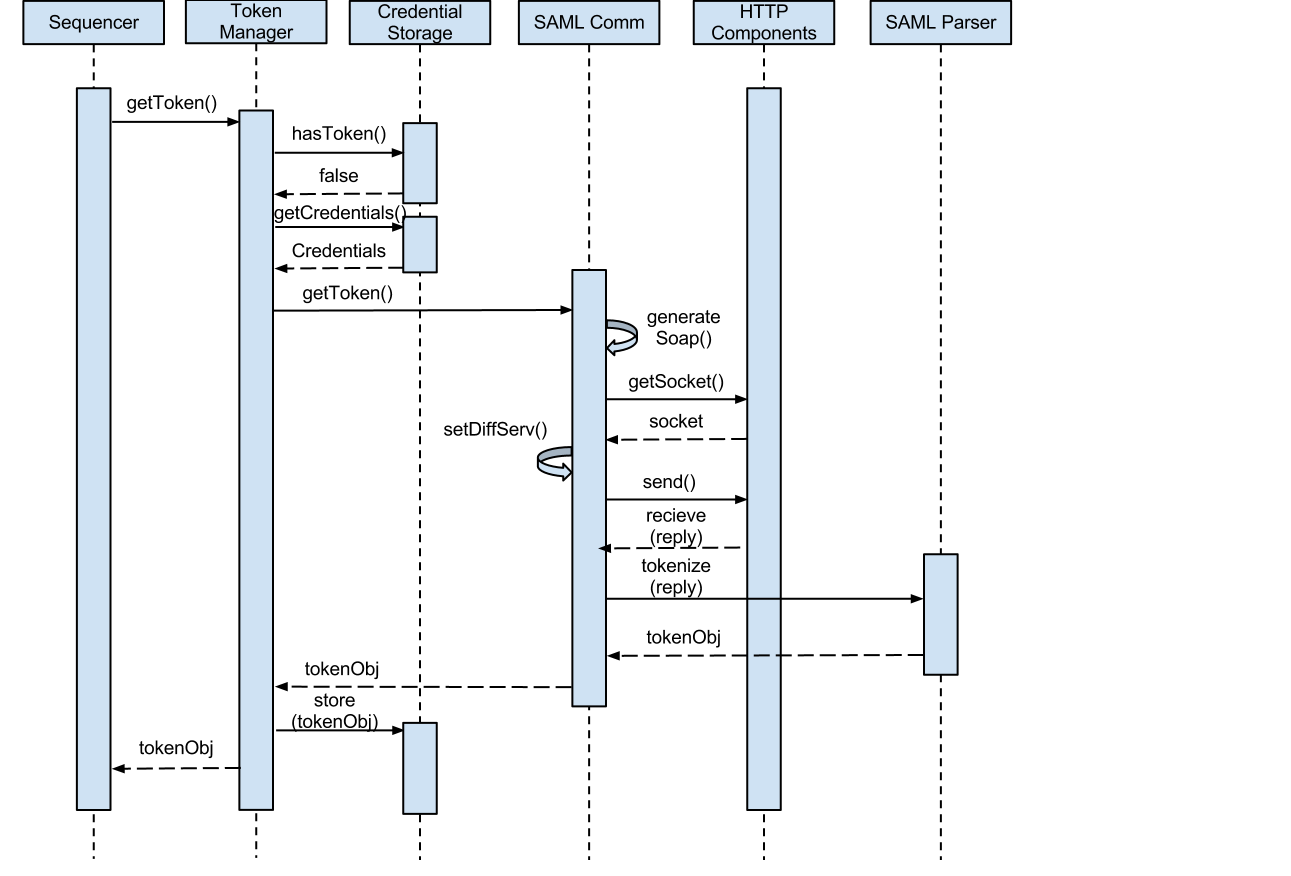
\includegraphics[scale=0.4, angle=-90]{CliSeqDiaGettingnon-storedtoken}
			\caption{Getting non-stored token}
			\label{fig:CliSeqDiaGettingnon-storedtoken}
		\end{figure}
		\begin{figure}[H]
			\centering	
			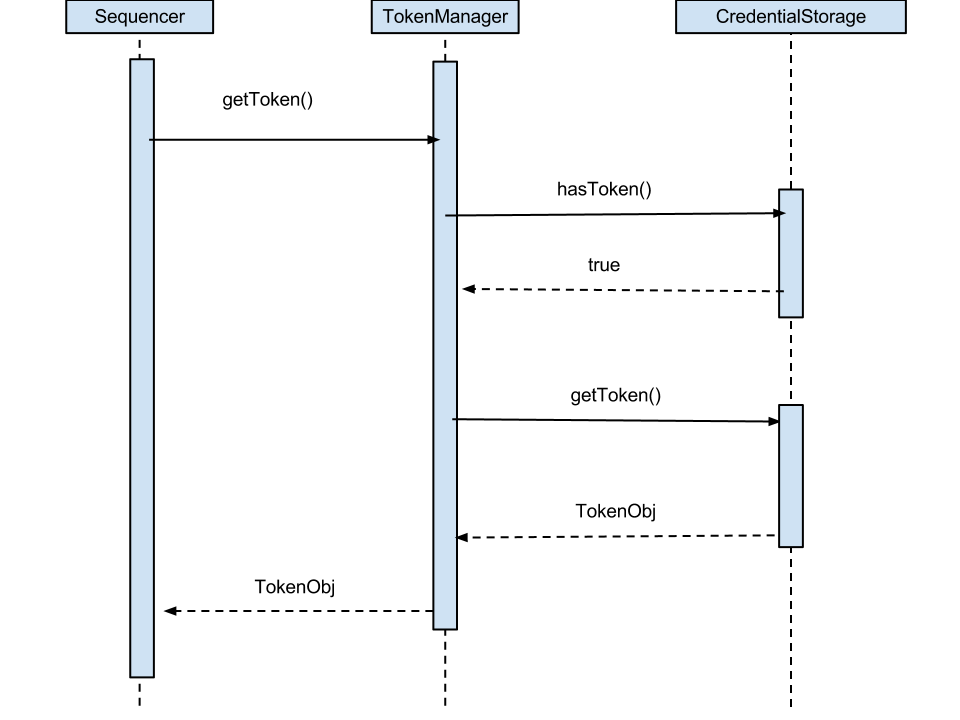
\includegraphics[scale=0.4, angle=-90]{CliSeqDiaGettingStoredToken}
			\caption{Getting stored token}
			\label{fig:CliSeqDiaGettingStoredToken}
		\end{figure}
		\begin{figure}[H]
			\centering	
			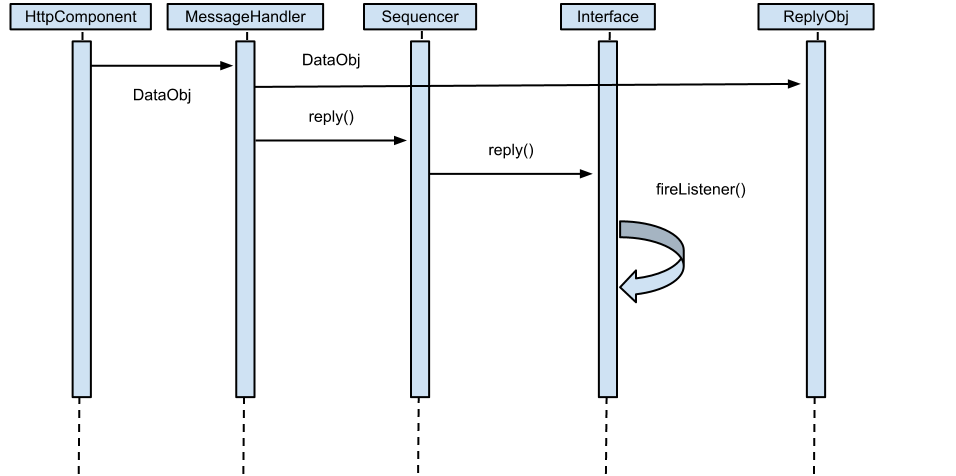
\includegraphics[scale=0.4, angle=-90]{CliSeqDiaReceivereply}
			\caption{Receive reply}
			\label{fig:CliSeqDiaReceivereply}
		\end{figure}
	% this sequence diagram might be better structured. Maybe with arrows happening first to be closes to echother. 
		\begin{figure}[H]
			\centering	
			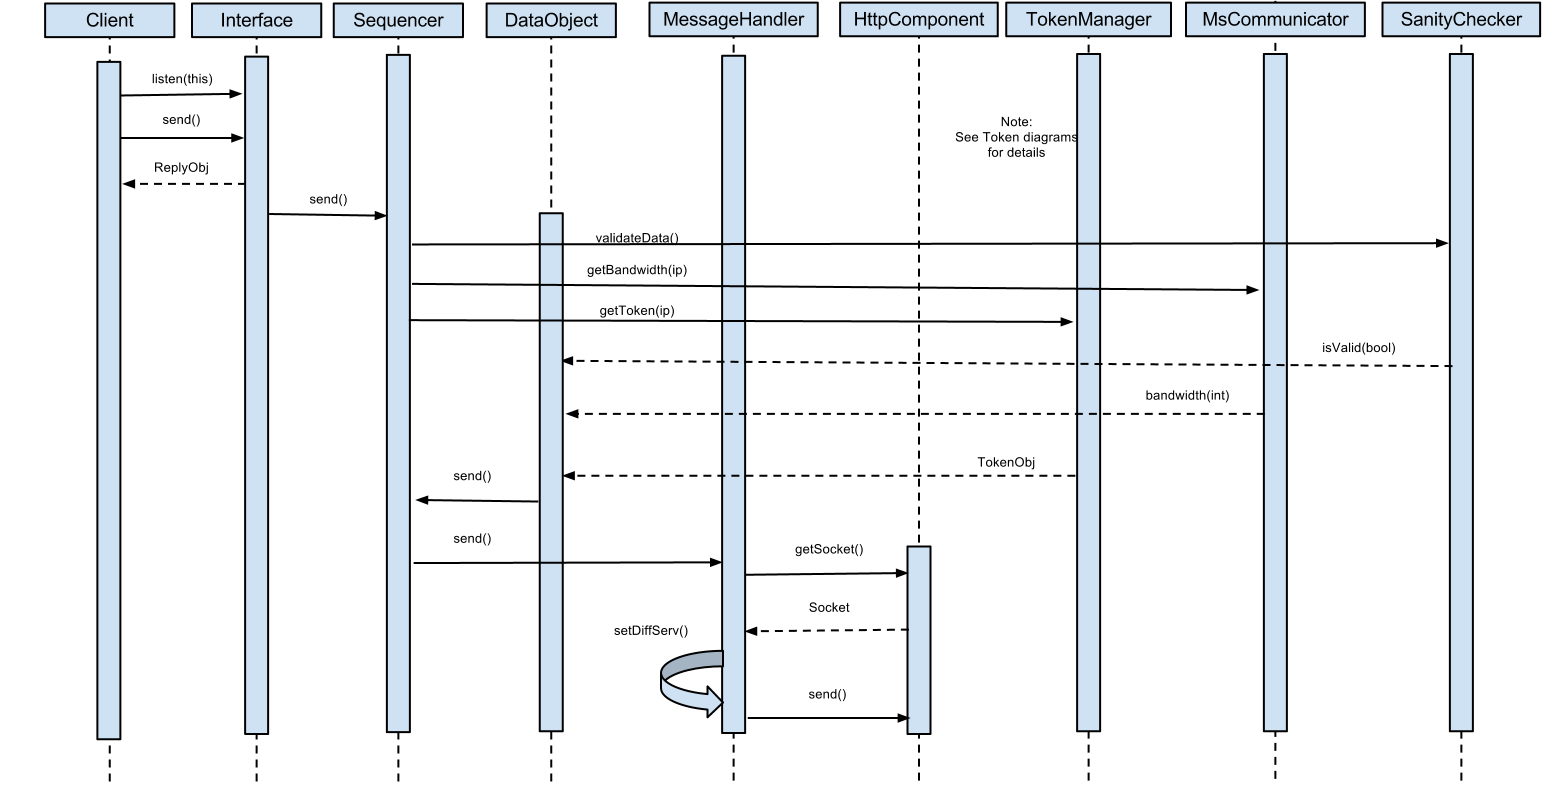
\includegraphics[scale=0.4, angle=-90]{CliSeqDiaSendData}
			\caption{Send data}
			\label{fig:CliSeqDiaSendData}
		\end{figure}

		


        \subsection{Server Side}\label{Server Side Design}

    In this chapter we are going to introduce the design, configuration and modification that we have done to the server side. In section \ref{Server Introduction} we will introduce the framework that we have built upon and what we are going to do with it. Next follows use cases, \ref{Server Use Cases}. Section \ref{Description of ESB concepts} will go into more detail about what the framework consists of. The section will also guide you through the basic processing units which is used in the framework. The next section, \ref{Textual Server Dataflow}, contains the dataflow through the server side, which will help you get a good overview of our thoughts about the design. \ref{Extensions to the ESB} goes into detail in describing our custom components in the framework, and together with the dataflow should give you a good understanding of the whole server side. Together with section \ref{Server Sequence Diagrams} you should get good system overview. Section \ref{Configuration of the ESB} will give you the 
details about how we have configured the framework, it will not contain description of how we have set variables during testing, but using this description should make it possible to get the framework up and running. The last section, \ref{Modification of the ESB} will depict how we have modified the framework to be able to meet our requirements, with this section you should be able to tell what modifications were needed and how we have altered those pieces. 

    \subsubsection{Introduction}\label{Server Introduction}
    The server side architecture consists of several components, the WSO2 ESB, the Monitoring Service and the GlassFish server. The GlassFish server is not necessary to modify and the MS is something we must assume exist in the network. The ESB is what we have to modify, configure and extend to meet our requirements.

    The ESB will be used to implement QoS for the web services. To do this, it will have to communicate with the MS, in addition to the clients and the services. The ESB must be configured to work as a proxy for the services on the GlassFish server. It will also be configured to use certain mediation sequences for incoming requests and outgoing responses. The extensions to the ESB consists mainly of custom mediators used in the mediation sequences. These mediators will have the tasks of determining priority of messages, contacting the MS for bandwidth data, and enforcing the priority. There will also be made modifications to one of ESB's library source code to allow setting the DiffServ field in the IP header.
    
    \subsubsection{Use Cases}\label{Server Use Cases}
    This section will outline the use cases that we have thought of in relation to the server side. With the help of these you should get a rough idea of what we want the server side to be able to do.\\\\
    \textbf{Title:} Request mediation\\
    \textbf{Requirements:} 3, 7\\
    \textbf{Actors:} Client, ESB, GlassFish\\
    \textbf{Main}
    \begin{enumerate}
        \item Client sends SOAP message with SAML Token to ESB proxy
        \item ESB extracts SAML token to get the client role
        \item ESB removes SAML metadata from message
        \item ESB adds metadata to message context.
        \item ESB sends message to GlassFish endpoint
    \end{enumerate}
    \textbf{Extensions:}
    \begin{itemize}
        \item[] 2a. SAML Token is invalid
        \item[] 2b. ESB sends error message to client
    \end{itemize}
    \textbf{Precondition:}
    \begin{itemize}
        \item Client is connected to ESB
    \end{itemize}
    ~\\
    \textbf{Title:} Response mediation \\
    \textbf{Requirements:} 2, 3, 7\\
    \textbf{Actors:} Client, ESB, GlassFish \\
    \textbf{Main}
    \begin{enumerate}
        \item GlassFish sends message to ESB
        \item ESB sets priority metadata in message context and SOAP header.
        \item ESB retrieves bandwidth information (See Monitoring Service communication use case)
        \item ESB prioritizes message (See Prioritize message use case)
        \item ESB sends message to Client
    \end{enumerate}
    \textbf{Extensions:} \\
    \textbf{Precondition:}
    \begin{itemize}
        \item Request mediation
    \end{itemize}
    ~\\
    \textbf{Title:} Monitoring Service communication\\
    \textbf{Actors:} Monitoring Service(MS), ESB\\
    \textbf{Main}
    \begin{enumerate}
        \item ESB requests bandwidth information from MS to a specific address
        \item MS returns bottleneck bandwidth to the ESB, as well as the address of the last Tactical Router before the endpoint.
    \end{enumerate}
    \textbf{Extensions:}
    \begin{itemize}
        \item[]	1a. ESB specifies an invalid address
        \item[]	2a. MS returns no information
        \item[]	2b. Address is in the same sub net as the ESB
    \end{itemize}
    \textbf{Precondition:}
    \begin{itemize}
        \item Response mediation
    \end{itemize}
    ~\\
    \textbf{Title:} Prioritize messages\\
    \textbf{Requirements:} 2, 6, 8\\
    \textbf{Actors:} ESB\\
    \textbf{Main}
    \begin{enumerate}
        \item ESB acquires QoS information through settings
        \item ESB adds QoS information to the SOAP header of the message
        \item ESB sets DiffServ field in IP header
    \end{enumerate}
    \textbf{Extensions:}\\
    \textbf{Precondition:}
    \begin{itemize}
        \item Response mediation
        \item Monitoring Service communication
    \end{itemize}

    \subsubsection{Description of ESB concepts}\label{Description of ESB concepts} 

    In this section we will shortly describe some important concepts of the ESB and message mediation.

    A mediator is the basic processing unit in \gls{synapse}\footnote{\gls{synapse} - An enterprise service bus}. Each message going through the ESB gets mediated through a sequence of mediators, which can be configured through either XML or WSO2’s graphical user interface. As long as the mediator inherit from a Synapse interface, any custom mediator can be used in the same manner as the built in mediators. To control the flow of messages through the ESB, there are two paths that can be controlled, the “in sequence” and the “out sequence”, which can also be configured to only apply for certain endpoints.

    The ESB is built around the notion of a message context, this object contains all the information regarding the message and the context around it. In the message context we can add properties, manipulate the message itself and manipulate the sending streams of the message. All the properties added during the receiving of a message is also added to the outgoing message, which we can use to our advantage.

    Each mediator in the sequence get access to the message context of the incoming or the outgoing message and can thus manipulate the context to its liking. When the mediator is done with the work it is supposed to do, it either calls the next mediator, sending it the possibly altered message context or returning true to indicate that the work is done.
    
    As you will soon see, we have taken full advantage of the modularity in the ESB. This means that even though much of the functionality in our mediators could be moved into one or two mediators we have decided to make many. For us this means much easier testing of each component and it gives each mediator a better defined role. For our customer this means an easier setup where they can mix and match each mediator and easily create custom sequences with just the functionality they need.

    \subsubsection{Dataflow}\label{Textual Server Dataflow} 
        This section describes the data flow through the ESB with the help of two diagrams. As a bonus, these diagrams show the general architecture of the server side very well.
\\
        \begin{figure}[h]
            \centering
            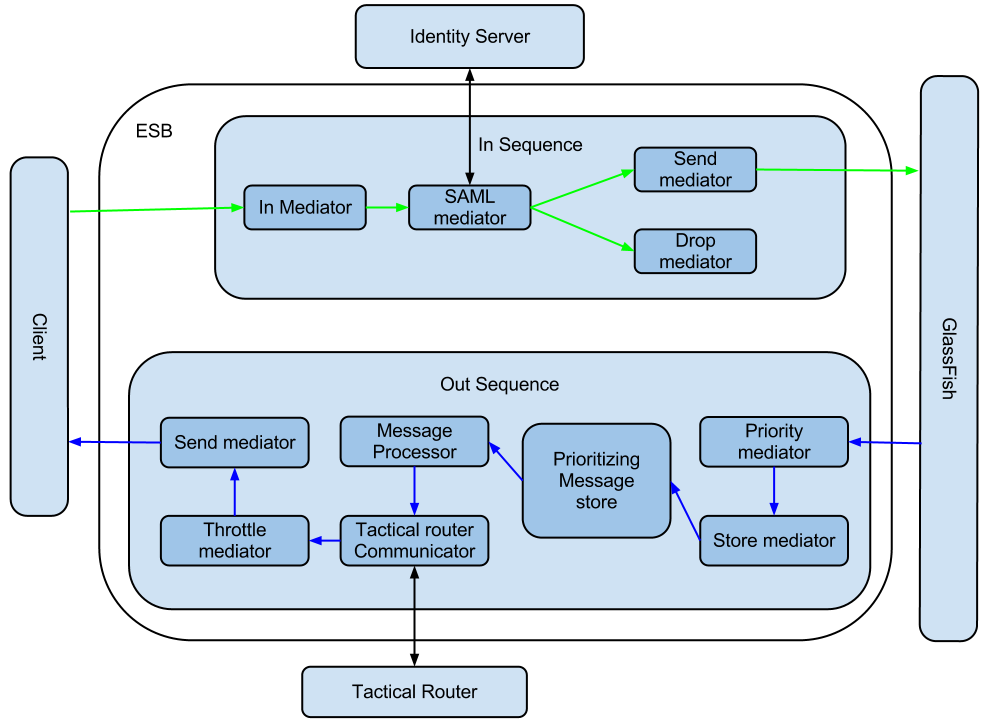
\includegraphics[width=\textwidth]{DataFlowDiagramServer}
            \caption{Server Data Flow}
            This diagram displays how the date flows through the server side. 
            \label{fig:DataFlowDiagramServer}
        \end{figure}
\\
Service Request :\\
To follow this flow, follow the green arrows in figure \ref{fig:DataFlowDiagramServer}. The ESB receives a request message from a Client, it is then sent to the SAML mediator, and then to the InMetadata mediator which when done sends it to the service endpoint on the GlassFish server, and the flow is over.
\\\\
Service Response:\\
To follow this flow, follow the blue arrows in figure \ref{fig:DataFlowDiagramServer}. The ESB receives a response message from the Service, it is then sent through a sequence of mediators, first the OutMetadata mediator, SoapPriority mediator, MS mediator and then  the Store mediator. The Store mediator stores the message in the Prioritized Message Store. The message is stored until the Sampling Message Processor picks it out before sending it on to another sequence of mediators. First in the sequence is the DiffServ mediator, then the Throttle Mediator and finally the Send mediator. The send mediator sends the message back to the client and the flow is completed.
\\
    \begin{figure}[h]
        \centering
        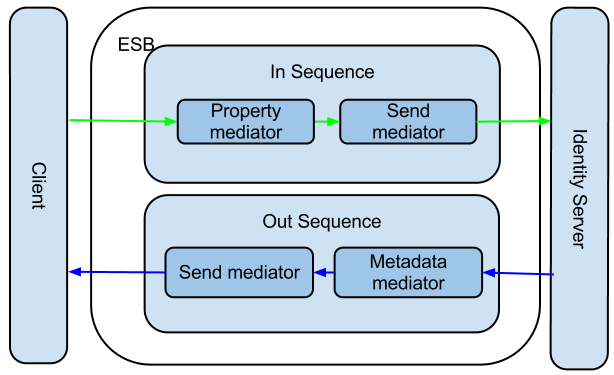
\includegraphics[scale=0.5]{SAMLauthenticationflow}
        \caption{SAML Authentication Flow}
        This describes the flow of an authentication request. 
        \label{fig:SAMLauthenticationflow}
    \end{figure}
\\           
SAML Authentication Request:\\
This flow is shown in figure \ref{fig:SAMLauthenticationflow}.The ESB receives a request (from a Client) directed at the dummy Identity Server, the ESB then uses the SendBack mediator to send the same message it got in back. The message then travels to the Out sequence where it gets a priority, a DiffServ value and some metadata gets added to the header of the message. The reason why this is done is explained in the section [TODO: Add reference to Identity Server problems here].%TODO fix

    \subsubsection{Extensions to the ESB}\label{Extensions to the ESB} 
    This section will contain a textual description of all the mediators used in the ESB. First we will describe all the custom mediators and then a short description of the built-in mediators we will use. All of our custom mediators have an accompanying sequence diagram to give a detailed overview of their inner working.
\\\\
\textbf{Custom mediators:}\\\\
SAML mediator:\\
    This mediator retrieves the user role from the SAML authentication and set this as a property in the message context. The service is retrieved from the 'recipient' field also found in the SAML authentication and added as another property. Depending on the configuration of the ESB this mediator can also detach the SAML authentication if this is no longer needed.
\\\\
InMetadata mediator:\\
	This mediator adds the IP of the client to the message context, which is done in order for the MS mediator to do its work. It will also set the Time-to-Live values in the message context if this is present in the SOAP header.
\\\\
OutMetadata mediator:\\
    This mediator retrieves the client role and service properties from the message context. These properties are then used along with a persistent registry to infer a priority for the message, and what the DiffServ field in the IP header should be set as. The priority and DiffServ values are then set as new properties in the message context.
    The DiffServ property in the message context will be used in the synapse core to set the DiffServ field before sending the message (See \ref{Modification of the ESB}).
\\\\
SoapPriority mediator:\\
	This mediator adds the DiffServ value and the priority as two custom SOAP header items. We use these fields on the client side in order for the clients to use the same DiffServ value.
\\\\
MS mediator:\\
    This mediator retrieves the \gls{ipaddress}\footnote{\gls{ipaddress} - A numerical label assigned to each device connected to the Internet} of the receiving client from the endpoint reference in the message context. It sends this IP address to the Monitoring Service and gets the IP address of the last Tactical Router on the path to the client, as well as the limiting bandwidth on the path. The mediator then sets this information as properties in the message context before sending the message to the next mediator.
\\\\
Prioritized Message store:\\
    This is not a mediator, but it is an important part of the response mediation sequence. This is a message store that stores messages in a priority queue. The queue is mainly ordered by the priority property of the message context, and secondly by the time when added. When retrieving messages from this store, the message on the top of the queue is returned. This ensures that high priority messages are processed before lower priority messages.
\\\\
DiffServ mediator:\\
	The DiffServ mediator sets the correct DiffServ value on the Socket. The DiffServ value is retrieved from the same value as the OutMetadata mediator put in earlier. Since correct use of DiffServ was very important to the client this mediator also does extensive logging which is important to look at when debuging.
\\\\
Throttle mediator:\\
    This mediator is used to ensure that high priority messages are sent first, by disrupting already sending messages, and it tries to ensure that the network is not being overflowed by this server by holding back messages. To determine what to disrupt and what to hold back, and for how long, several properties are used; the priority of the message, the available bandwidth, the IP address of the client side Tactical Router, and the real time demand of the request. In order to do this, the mediator must keep a list of sending messages and where those messages are going.
\\\\
SendBack mediator:\\
    This mediator sends the message back to the client, but before it is sent it is mediated through the out sequence of the ESB.
\\\\
\textbf{Built in Mediators:}\\\\
Send mediator:\\
    This is a built in mediator that sends the message to an endpoint (the requested service).
\\\\
Store mediator:\\
    This is a build in mediator that stores the message context in a message store, here this is the Prioritized Message store.
\\\\
Sampling Message Processor:\\
    This is not a mediator. It is a built in class that takes messages out of the Prioritized Message Store at a defined interval. And then sends them to a mediator sequence, here starting with the DiffServ mediator.

    \subsubsection{Sequence Diagrams}\label{Server Sequence Diagrams}
    This section contains some sequence diagrams which you can use to get a more in depth look into the code and methods used in the mediators above. The diagrams may not reflect the actual method names or display the full complexity of the code, but they should be sufficiently detailed that it should be possible to recognize them in the code.
    
        \begin{figure}[H]
        % TODO: ref in text. 
            \centering
            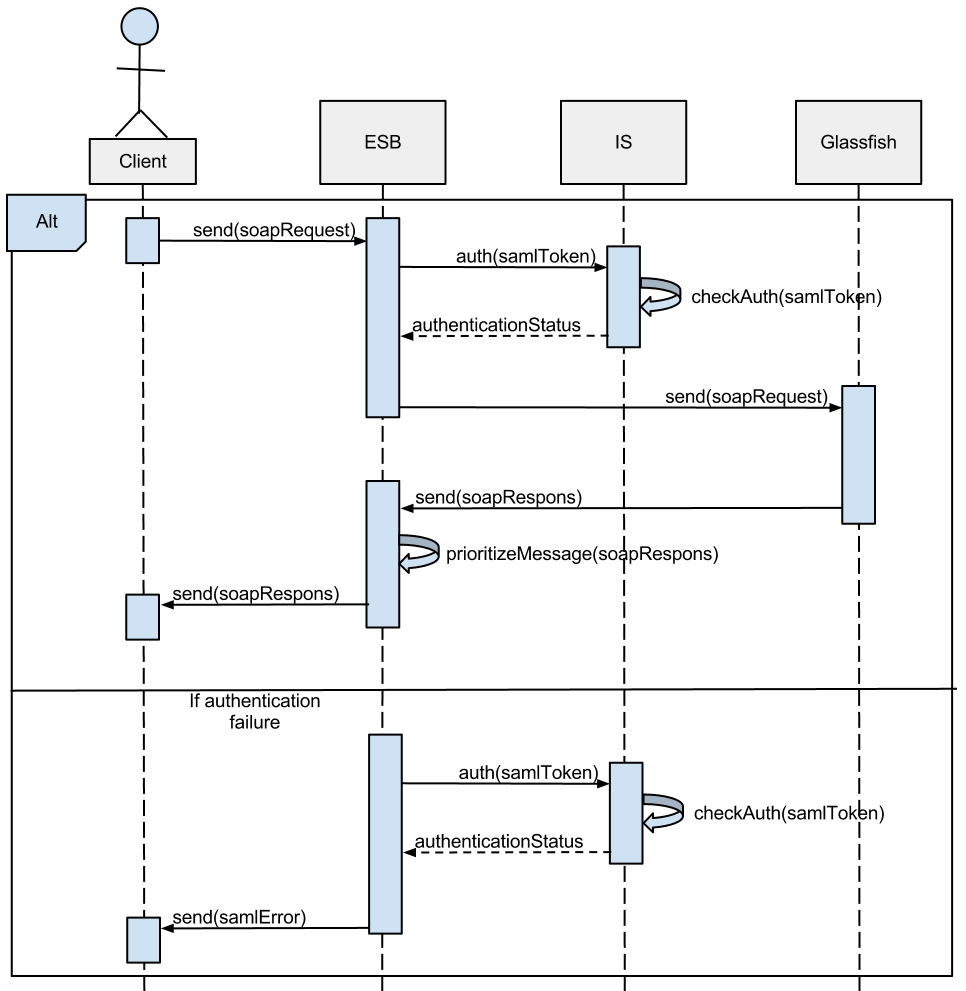
\includegraphics[scale=0.3]{System-levelsequencediagram}
            \caption{System-level sequence diagram}
            This high level diagram shows how the client communicates with web services through the ESB.
            \label{fig:System-levelsequencediagram}
        \end{figure}
        
        \begin{figure}[H]
        % TODO: ref in text 
            \centering
            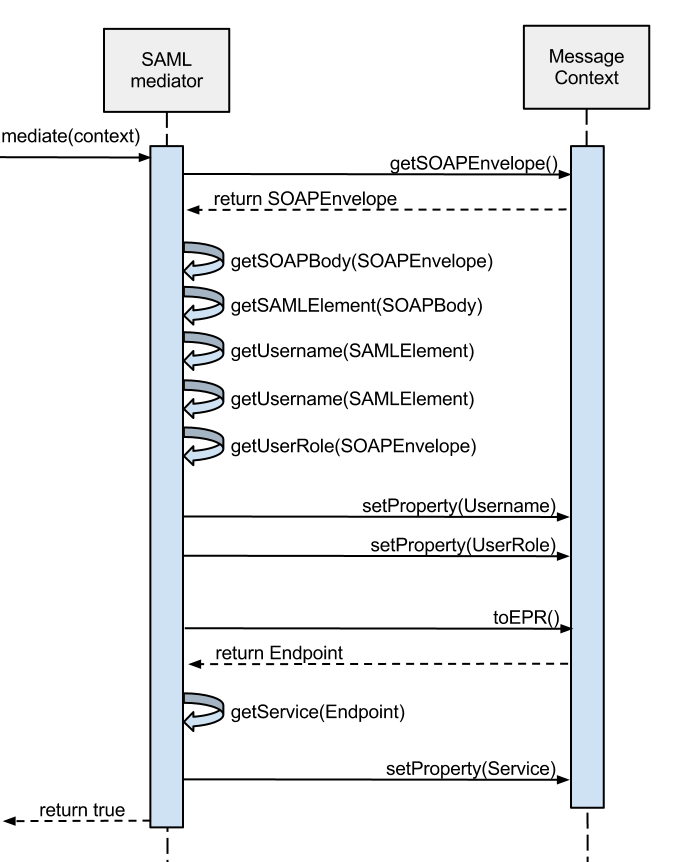
\includegraphics[scale=0.3]{SAMLmediator}
            \caption{SAML mediator sequence diagram}
            This diagram describes how the SAML mediator will get data from the message, and set it in the message context so it can be used later in the response sequence
            \label{fig:SAMLmediator}
        \end{figure}
        
        \begin{figure}[H]
        % TODO: ref in text 
            \centering
            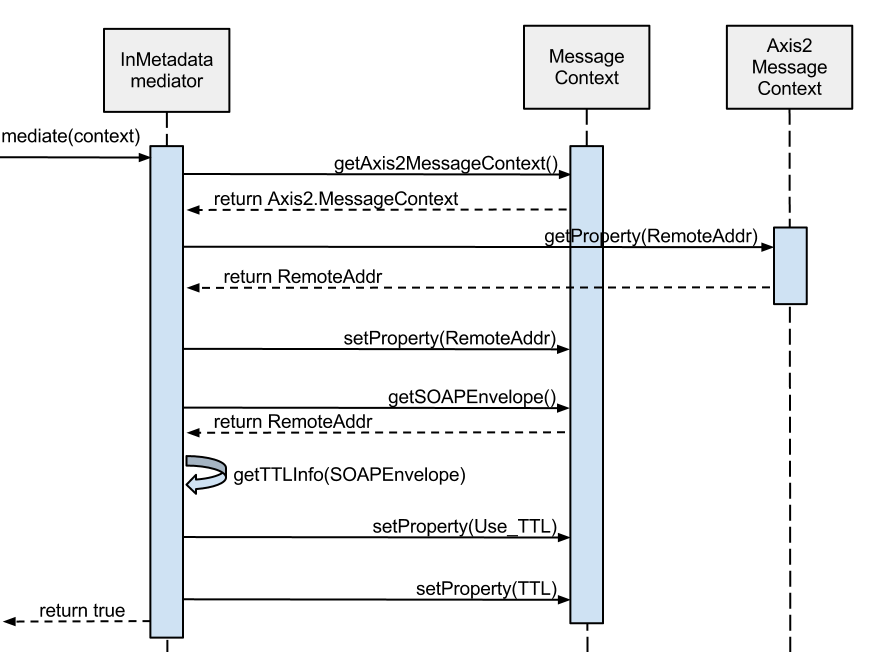
\includegraphics[scale=0.3]{InMetadatamediator}
            \caption{InMetadata mediator sequence diagram}
            This diagram shows how the InMetadata mediator works when it adds the IP address and Time-to-Live.
            \label{fig:InMetadatamediator}
        \end{figure}
        
        \begin{figure}[H]
        % TODO: ref in text. 
            \centering
            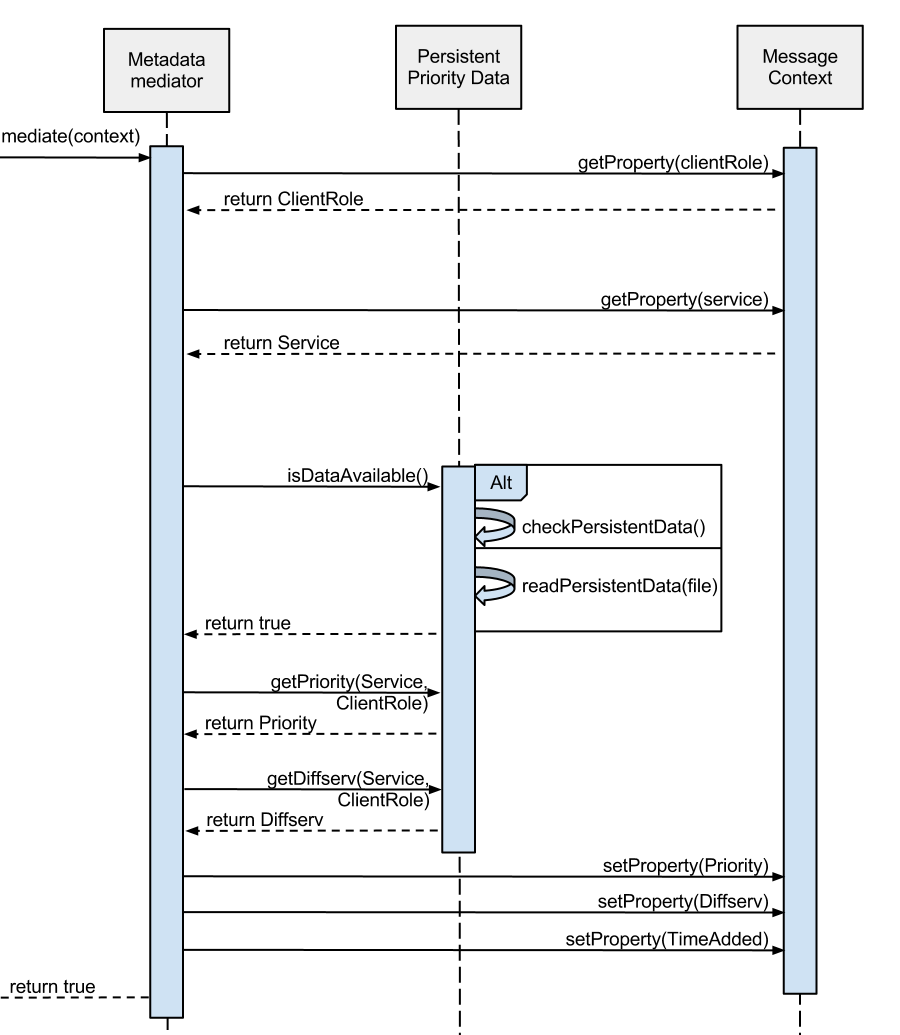
\includegraphics[scale=0.4]{OutMetadatamediatorsequencediagram}
            \caption{OutMetadata mediator sequence diagram}
            The diagram shows how OutMetadata mediator works.
            \label{fig:OutMetadatamediatorsequencediagram}
        \end{figure}
        
        \begin{figure}[H]
        % TODO: ref in text 
            \centering
            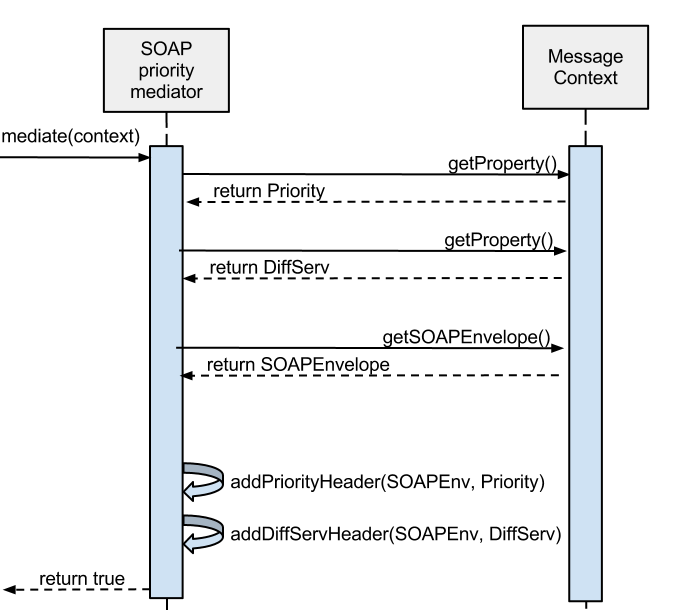
\includegraphics[scale=0.3]{SoapPrioritymediator}
            \caption{SOAP Priority mediator sequence diagram}
            This diagram shows the inner working of the SOAP priority mediator.
            \label{fig:SoapPrioritymediator}
        \end{figure}
    
        \begin{figure}[H]
        % TODO: ref in text. 
            \centering
            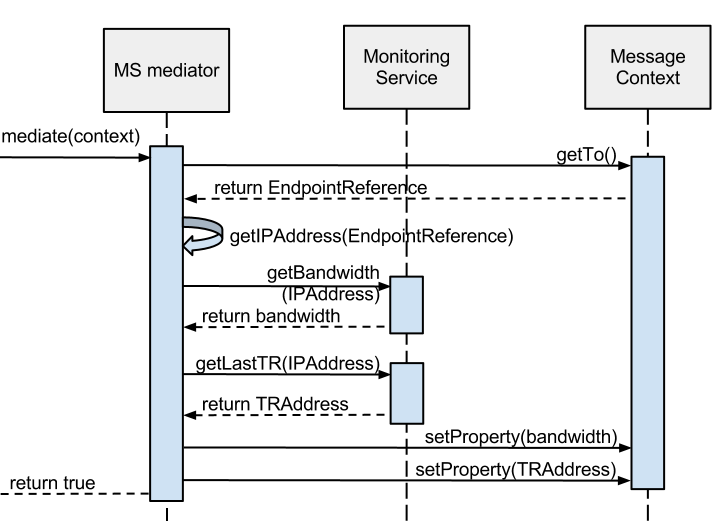
\includegraphics[scale=0.3]{MSmediatorsequence}
            \caption{Metadata mediator sequence}
            This diagram describes how the Metadata mediator retrieves previously stored properties from the message context, determines a priority for the message, and sets priority and DiffServ properties in the message context
            \label{fig:MSmediatorsequence}
        \end{figure}
        
        \begin{figure}[H]
        % TODO: ref in text 
            \centering
            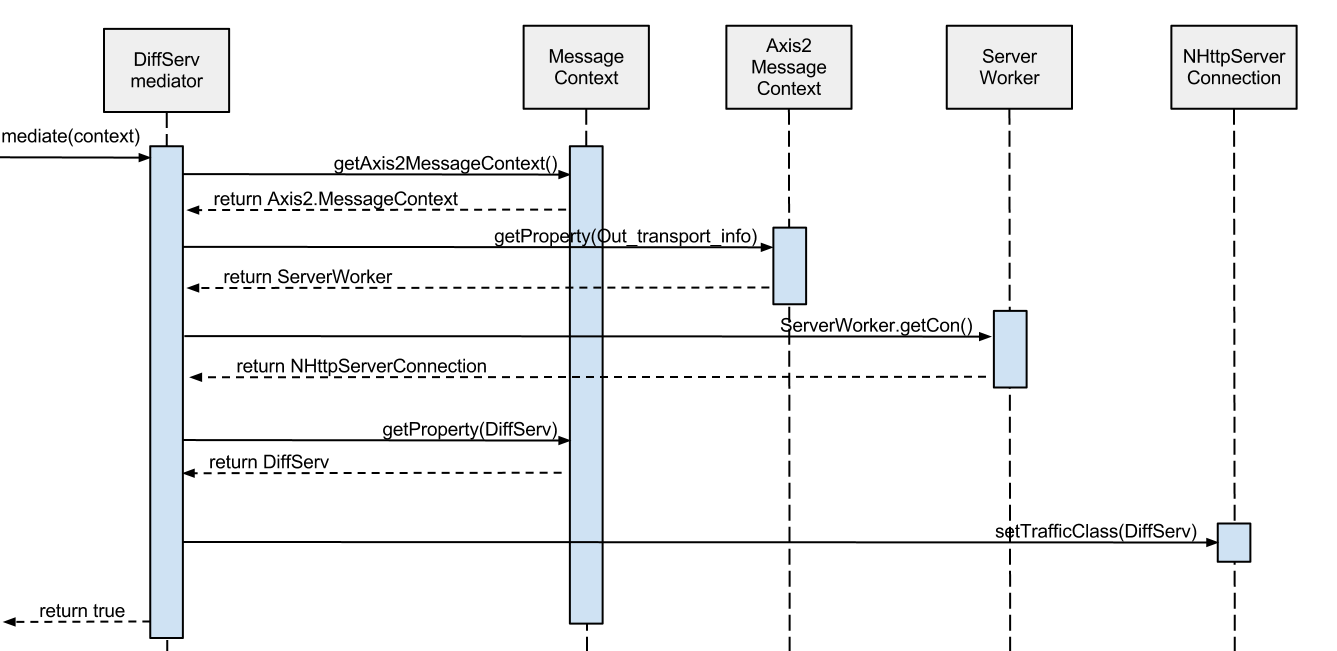
\includegraphics[scale=0.3]{DiffServmediator}
            \caption{DiffServ mediator sequence diagram}
            How we set DiffServ priority on the underlying Socket.
            \label{fig:DiffServmediator}
        \end{figure}
        
        \begin{figure}[H]
        % TODO: ref in text 
            \centering
            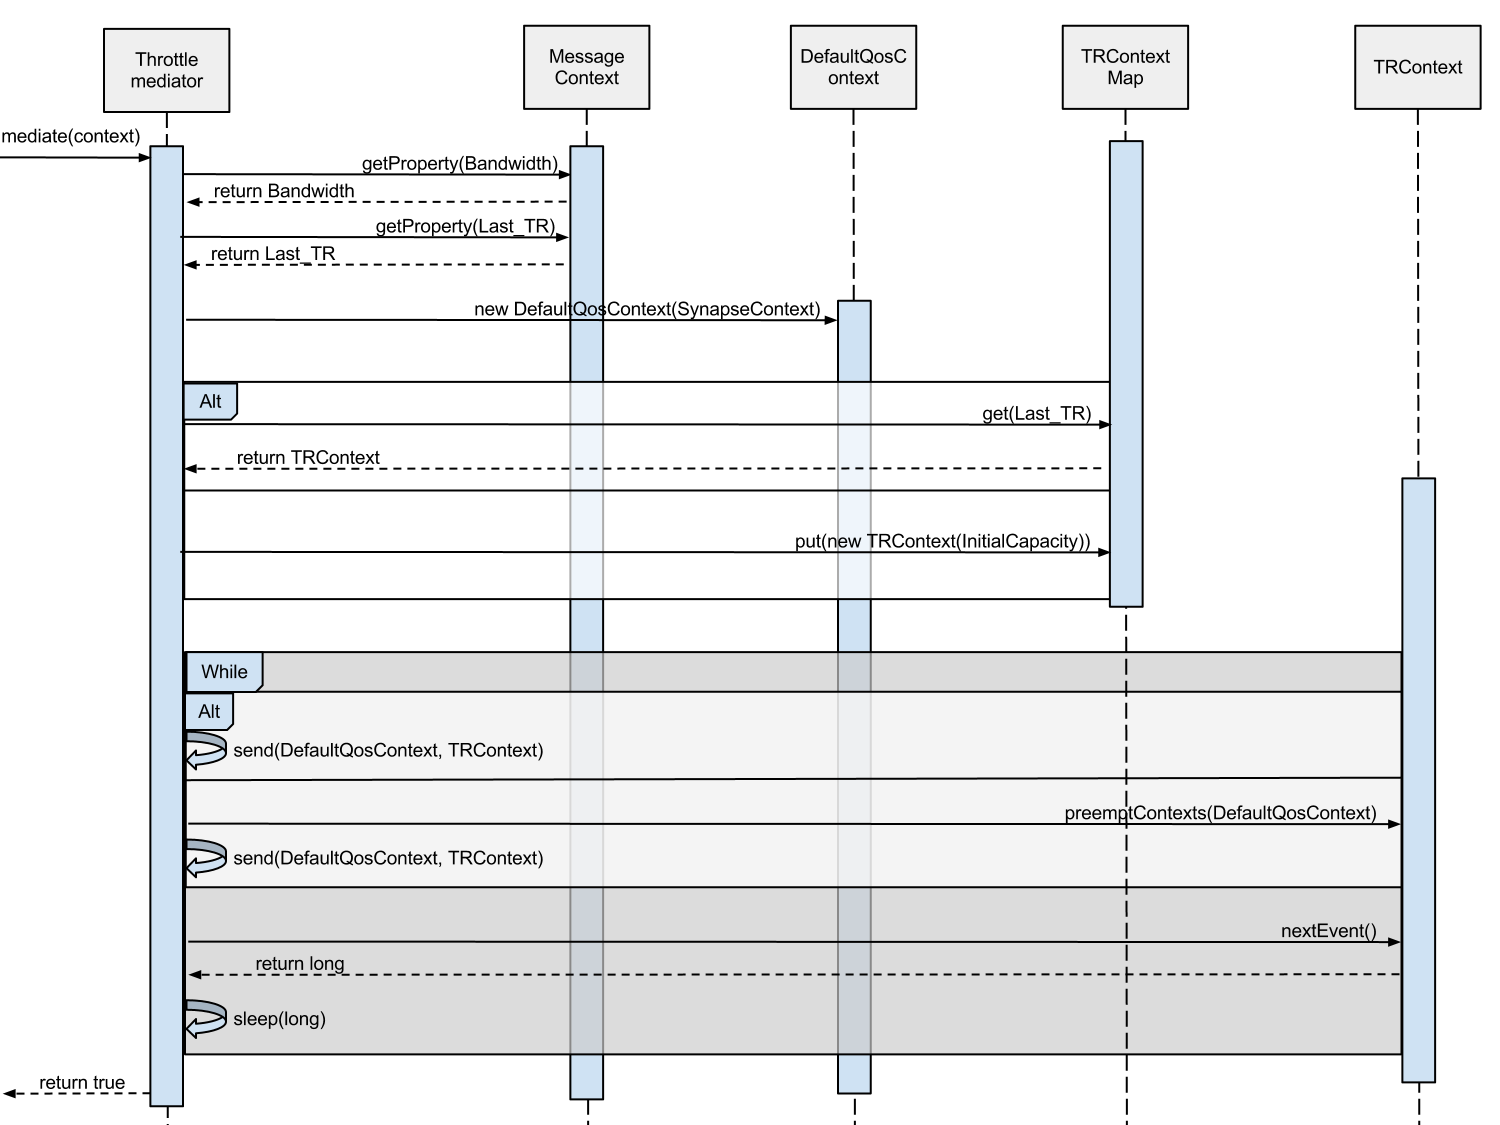
\includegraphics[scale=0.3]{Throttlemediator}
            \caption{Throttle mediator sequence diagram}
            The meat of the server side mediators.
            \label{fig:Throttlemediator}
        \end{figure}
        

    \subsubsection{Configuration of the ESB}\label{Configuration of the ESB} 
	In this section we will explain how to configure the ESB. For general configuration of the ESB, f.ex. configuring new services or WS-Discovery, please refer to the official WSO2 ESB or Apache Synapse documentation.

	\begin{shaded}
	It is highly recommended that you follow the appendix [TODO: add reference to appendix] for an in depth guide on how to setup the ESB with the needed modifications before you read this section.
	\end{shaded}

	First we will look at the file “ppd.xml”, which should now be in “/path/to/wso2esb/”, ppd is short for Persistent Priority Data. This file contains maps from “service name” and “client role” to “priority” and “diffserv”. Here “service name” should be the path to the service on the ESB, “client role” should be the name of the client’s role, “priority” is the internal priority we use in the ESB (higher is better) and “diffserv” is the value that will be set in the IP header on communications with the client. Both DiffServ and priority must be integers.
	The service element also has the useDefault property, which when set to true lets roles not configured in this file use values in the default role. When useDefault is set to false unconfigured clients will get a priority and DiffServ of 0. If useDefault is set to false there is no need to configure a default client for the service.
	Below is an example setup of a service in ppd.xml.\\

\lstset{language=XML}
\begin{lstlisting}[frame=single] %Ok to not have this referenced =)
<?xml version="1.0" encoding="UTF-8" ?>
<config>
   <services>
	   <service name="/services/EchoService" 
	   useDefault="true">
	         <client role="clientRole1">
	           <priority>100</priority>
	           <diffserv>10</diffserv>
	         </client>
	       <client role="Default">
	           <priority>321</priority>
	           <diffserv>8</diffserv>
	       </client>
	   </service>
   </services>
</config>
\end{lstlisting}\\

	Next we look at a file that is specific to our implementation of the MSCommunicator (Monitoring Service Communicator). Since our implementation does not actually have a monitoring service to contact we use the file “ms.xml” in “/path/to/wso2esb/” to configure data groups of destination IP, name of last Tactical Router before client and the bandwidth capacity of the ‘weakest’ link on the path measured in KBps. Below is an example configuration.\\

\lstset{language=XML}
\begin{lstlisting}[frame=single] %It is ok that this is not referenced in text =)
<?xml version="1.0" encoding="UTF-8" ?>
<config>
   <RoutingInfos>
	   <RoutingInfo>
	       <destIP>127.0.0.1</destIP>
	       <lastTR>bob</lastTR>
	       <bandwidth>0.2</bandwidth>
	   </RoutingInfo>
   </RoutingInfos>
</config>
\end{lstlisting}\\

	If the MSCommunicator is modified to communicate with a Monitoring Service this file will not be needed anymore.

	The last file we will look at is synapse.xml (\ref{attachment:server config}), which should now be in “/path/to/wso2esb/repository/deployment/server/synapse-configs/default/”. This file contains configuration for proxies, endpoints, message stores, mediation sequences, and more. The important things here are:
	\begin{itemize}
	\item the sequence qos, where we can find the configuration for the Throttle mediator. Here we can set the properties minBandwidthPerMessage (integer measured in Bps) as well timeout, which is the longest time a message will be allowed to try sending (integer measured in ms) before it is discarded.
	\item and the messageProcessor, where the parameter interval can be set, this determines how often a message should be taken out of the message store, measured in ms.
	\end{itemize}
	Other things in this file should mostly be untouched, as they define what the ESB does with messages, most of which is needed to do the prioritizing and throttling.

	The ESB can also be configured through its web interface on https://ADDRESS:9443/carbon

    \subsubsection{Modification of the ESB}\label{Modification of the ESB} 
		The WSO2 ESB source code will have to be modified to allow for setting the DiffServ field in the IP-header of packets sent. The idea is that we will set a property, DiffServ, in the message context, and let the DiffServ mediator retrieve this property and set it on the socket used for sending.

The source code for all the dependencies of WSO2 ESB is included in its source code. As such we only altered files in this source. This made it easier for us to build and create a runnable instance of WSO2’s ESB. To also try and support future versions of Apache Synapse and WSO2 we have also pushed the changes upstream, which should mean that in the future WSO2 will support setting DiffServ by default.    


\section{Implementation}\label{Implementation}
    [The specifics of the implementation of the sollution.]

\section{Testing}\label{Testing}
    [The testing setup and suite. The testing method and how we did the testing.]
    
    % describe the test suit NS3
    
    % write about the choise of of JUnit tests. 
    
    % we have planned for two tests and merg phases, which is to few, we have to do that every week. 
    
    % describe the testing procedure. 
        % here it would be natural to describe the whole testing pahse from unit testing to test suit to code review(as part of testing)
        
    % more?

\section{Results}\label{results}
    [A thurough presentation of the results of the project. The test results and other interesting findings for this project.]

\section{Conclusion}\label{Conclusion}
    This section concludes our work on this project and gives a summary of our accomplishments and results. It also gives an overview of the future work of the prototype that we created.
    
    % sumary of our accomplishments
    \subsection{Project accomplishments}\label{Project accomplishments}
    [Did we reach the goal?]
    
    TODO finish


    % future work section
    \subsection{Future Work}\label{Future Work}
    In this chapter we will discuss what can be worked on further and improved in the future. Some things we did not have time to do as well as we might have wanted, and some things that we knew would have to be made/modified later.
    
    \subsubsection{Server}\label{Future:Server}
        In our MS Mediator we use a dummy implementation of the MS Communicator, which just reads an xml-file with the needed data. A future work would be to make an implementation that acutally contacts a Monitoring Service and use this in the mediator.

        The throttling done in the ESB is relatively static, one configuration will work very well for some scenarios, but might not work as well for other ones. In the future, making it more dynamic might be desireable. The first thing to do might be to make and use a new implementation of the Message Processor instead of the built in SamplingMessageProcessor, retrieving a messages from the Prioritiezed Message Store dynamically instead of just once every predefined interval milliseconds could get you a long way. Also the Throttle mediator could be made more dynamic, for example by varying the now static variables based on percieved network load.

        If propper SAML authentication is implemented the IdentityServer proxys sequence would have to be modified as well.

\subsubsection{Client}\label{Future:Client}
As mentioned in the changes-secton (\ref{Changes}), the components related to authentication on the client side were not implemented as desired due to the problems with the Identity Server. Naturally, this is something that can be adressed in the future, when a proper IS is working.



\section{Project Evaluation}\label{Project Evaluation}
    During this last chapter before the conclusion, we will try to take a step back and look at the project. We will try to criticize were that is appropriate, and give our self a pat on the back when that is in order. We hope that after reading this, you will understand the problems we have faced and where we have gone wrong. And hopefully we can point out how we should have avoided those problems. This chapter will work as a summary over the process.
    
    \subsection{Task evaluation}
        % was the task well enough described? Or would it have been better if the task was stricter and had more requirements?
Our task was very focused on research, and with that came a lot of freedom to choose which technologies to use, and to some degree what to actually implement. We did manage to settle on some requirements quite early, although most of them were not very strict. Even so we felt this was not a problem and started designing. In the later parts of the project we realized having such loose requirements might have led us to bite over a bit much. Stricter prioritized requirements might have let us know what parts were more important than others, and we could have focused more on them. We realize we should have asked the customer for these stricter requirements on both what to use and what to implement.

Since the project was research focused from the customer side we got quite a lot of freedom when it came to the project. This freedom was not a hindrance for us, but we could have handled it better. As mentioned above the requirements we agreed on with the customer was a bit to loose, again here we should have realized that they gave us this freedom and we should have insisted on stricter requirements. When it came to testing the customer gave us the same freedom and again we should have used that freedom to write up some strict test requirements. In the end the freedom gave us all the choices, but we could have handled it better.

Overall, the task has been very interesting, and we are in general very happy with the result of it.

        
    \subsection{Team organization}
        % the flat structure worked out well
% we had no conflicts in the group. 
% the task distribution that automatically happened 
% comment on how this worked: some people had the unofficial responsibility for some tasks. Jan - IS, Jørgen - NS3, Ola - rooms, Magnus - Report, Stig - client. 
% evaluate the work schedule - mon-thur/10-16.
The problem we had with the roles in the group, is that we did not manage to switch betweeen them during the project. This resulted in some instances where we could not proceed with something, because the one who knew the most about it was ill. This was something that we were quite wary of in the beginning of the project, but we did not follow it up with the same care. The reason behind this is partly that it was usually easier to simply ask the person in charge of that specific part, to explain what you did not understand. Another reason was that we worked together every day during the project, which probably gave us the false confidence that we would not need to share the information. The few early roadblocks that we did encounter during the start up, where we could have done something about it, were probably so small that we just carried on without thinking about it.

We feel that the flat structure we chose worked out quite nice. When we came to a big decision that one of us felt uneasy about taking full responsibility for, we talked about it in the group, and came to a mutual decision. There are many reasons why this worked in our group, but a key enabler was the fact that we worked together Monday to Thursday. This close proximity made such decisions easy to approach, and agreement could quickly be made. If we had not had this work schedule, this sort of management might not have worked out the way it did.

We mentioned roles above, but we would also like to mention a bit about how that worked on a daily basis. Because we grew into certain roles as the project progressed, we also got some responsibilities. For instance, oneof us quickly became the main contact between the group and the supervisor, but having only one person handling that communication did not hinder use. In fact, the communication became quicker, because the supervisor could relate to one person and not everyone, and the fact that when someone in the group wanted to ask the supervisor about something, they could contact Magnus.

Luckily, we had very few conflicts in the group. There was some miscommunication which led to some disagreements, but there where very few of those. Among the few things that came up during this 15 week long project, was a miscommunication about when we were going to start working again after the Easter vacation. This little incident only lead to some stressful days, and the misunderstanding was cleared away.

As mentioned above, we tried to work together from Monday to Thursday from 10:00 to 16:00. This worked rather well during the whole project, except for some hiccups regarding the "early" start. We had some weeks where not all of us managed to get up in time, but after a meeting within the group we cleared away any bad air, and did not really experience any such hiccups after that.

        
    \subsection{Planning}
        % how the beginning was
In the first couple of weeks we spent a lot of time trying to understand the task and what needed to be done. We did not plan this process very well. This was probably because we did not know exactly what to plan for. What we did do was make daily agendas of what we should research.

After the first few weeks, we had managed to get a decent idea of what needed to be done, and so the more detailed planning began. We started by making a Gannt diagram (ref:Appendix \ref{attachment:file:Gantt} - gantt.html) with the different work packages we needed done by what dates. We should probably have planned in more detail at his point, and updated the gantt diagram when we learned more. In the end we did keep most of the deadlines we set: we started implementation when intended, and we only went a week past the intended deadline for implementation (excluding some important bugfixes). 

The biggest miss in the initial plan was probably that we intended to have the final report ready by April 16th, so that we could get detailed feedback on it before the final delivery. This ended up not happening because implementation required more resources than anticipated, and we prioritized the product before the report. We did not think of this as a problem, as we knew that we would get good feedback from our customer, supervisor and possibly some other people.

We also started making weekly Activity Plans (ref:\ref{}), instead of the daily agendas. The first two weeks of activity plans were very badly done, and not included in the report. But after that we made more detailed and more accurate plans.

Work breakdown structures were also made. They started out somewhat inaccurate, but by the end of the design phase they had become more correct and informative. 

Time estimation on the different tasks in the activity plans were, as always, very difficult. Some tasks ended up taking more than twice or even three times as much time as anticipated, while other tasks ended up taking less than half of what was planned. But most of the time we were within 30\% of the anticipated time, which we believe is pretty good.

Towards the end of the project, with bug hunting and finalizing the report, we ended up not making activity plans. We did not make plans for bug hunting because bugs are generally hard to anticipate. But the report writing could probably have been planned better.
% How we continued and adapted our planning
% going from the daily documents to activity plans.
% time estimation    
% Activity plans - how they worked out. 
        
    \subsection{Methodology}
        % Scrum 
% Agile
% Did the metodology work for us?
% Could we have adapted better to our methodology?
In this project we went against the current when it comes to modern software development methodology. Instead of going with the darling of the development world, SCRUM, we chose to go back and pick something that most would not. The waterfall model might not be the best fit for everyone, but for this project we think we got it right.

The first thing we knew was that most of the technologies was unfamiliar for everyone, even the customer, this meant that we had to invest a lot of time getting to know the different frameworks. Another thing was the research focus of the project, which demanded a certain investment into planning. All this lead us to the waterfall model, explained in section ~\ref{Software project life cycle}, which worked out quite well. We had a large planning phase, which included some head-scratching moments, but for the most part, we got through it. The implementation phase had some more problems, mostly with regards to time estimates and external dependencies. Had we gone for a more agile methodology, we might not have ended up with such a thorough design.

Although the previous paragraph does mention that we chose the waterfall model, we did not completely forget the agile world. Most of the implementation went according to a more agile development methodology, where we had weekly sprints, tried to have code reviews and used unit testing. We feel that this mixing of methodologies is some of the things we excelled at the most during this project. The waterfall model helped us with the planning and design of an unknown entity, and the agile implementation lead to cleaner and better code quality.

        
    \subsection{Meetings}
        % What worked? 
% What did not?
% Supervisor meetings was kind of meaningless in the beginning. 
% FFI meetings did occure frequently and smoothly. 
% FFI meetings mostly gave us a good relationship with the customer. The actual information shared and the topics discussed would have been equally good or better discussed by email. 
        
    \subsection{Communication}
        
\indent \indent \textbf{Group communication} \\
The communication inside the team worked well, because we were working in the same room most of the time. This contributed to the prevention of conflicts. We also had some "Team building" that helped us not get on each others nerves. Other than that we used SMS to keep in contact with each other outside of the university. This resulted in quite a good team spirit and there were no major mishaps regarding communication inside the group.
\\

\textbf{Supervisor communication} \\
The overall communication with the supervisor has been as expected. Some times there would have been nice with an answer to some of the emails about meetings. Typically we ask the supervisor for a meeting, decide time and place, and the supervisor doesn't confirm the meeting time, but he shows up so there is not really a problem. Other than that we had a good rapport with the supervisor and he always answered our questions. He was particularly good at helping us with the report, guiding us on how to lay it out and explaining what a good report should contain. There was very easy dealing with him as we could just send him an email or even meet him at his office.

For the most part our meetings with him went quite well except for one little communication error which we did not present clear enough to him. In the start of the project we were not quite sure what development methodology we were going to use and as stated earlier we eventually went with a modified waterfall model. The supervisor recommended SCRUM and was quite supportive of that way of developing. The problem arose when we did not convey clearly to him that we had chosen waterfall and some of the meetings ended with some confusion because of this. But we took it up during a later meeting and straighten every thing out.

The biweekly meetings with the supervisor worked well and we could always count on some insight into the problems we had faced. We also received good feed back on the weekly reports, activity plans and schedules which we sent.
\\ 

\textbf{Customer communication} \\
Since the customer was located in Oslo we had quite a challenge when it came to communication. Early on we decided together with the customer that we wanted to do weekly meetings over Skype. This worked out very well and we got lots of feedback over Skype. The customer did not mind us sending a lot of emails either, meaning that a lot of communication went over email which worked out very well. We got feedback when we needed it and we resolved problems either over email or, if the subject needed some discussion, at the weekly meeting. The customer also gave us very good feedback on the report which indicated their level of commitment. 

In addition to all this they also made several trips to Trondheim where we would have face to face meetings. This worked quite well, but we did not always prepare the way we should or could and some of the meetings were quite short for a trip from Oslo to Trondheim. But this level of commitment from the customer really impressed us and we are quite grateful that they gave us this opportunity.
\\


        
    \subsection{Design phase}
        Since the project contained such a large design phase it is only natural that we elaborate on what that phase entailed.

We started the design phase with a vague idea about what we were going to create. With the help of the customer we got a little further and soon we were going strong. Because of the nature of the project we did not have a clear starting point. So in the beginning we followed every hint that the customer gave us and tried to use every framework that the customer said could help. This gave us a lot to do because we had to get familiar with a lot of frameworks and asses their usefulness for the project. We then came up with the design which you can see in the prestudy section~\ref{Server side Architecture} and \ref{Client side Architecture} which we used as a spring board into the actual design.

After this initial design we first checked with the customer that the design was something like what they had in mind and then went forward with our design to come up with a more final version. Since we had gotten a little more confidence in the design we started putting more effort into the different frameworks that we wanted to use and developing a better image of what we could create.

The design phase went quite well, and the only real problem we had were problems related to unfamiliarity with the frameworks we decided to use. These problems subsided over time as our familiarity grew.

Most of what we decided during the design phase were possible, but some things were out of our reach. Among other things the design of the testing suite had to be scaled back quite a bit, but everything that we had to alter during implementation were thoroughly discussed with the customer so that they had a saying in every alteration.

The design phase overall were quite helpful and since we initially had no idea about how the final design would look the large design phase really helped. We learned a lot during those weeks and we have a new understanding of what is required during design for a large scale project such as this.

        
    \subsection{Implementation phase}
        % we might have been a bit slow to get to the coding part but it worked out well(?). 
% did we complete implementation on time?

Because of all the research needed for this project we planned to start the development phase relatively late in the project. And we did manage to start it at the planned time. We had quite a lot to do during the implementation and because of the frameworks we worked with we had to familiarize us with the code of these as well. 

On the server side of the project we quickly saw that most of the implementation would take less time than originally anticipated. That way we could start looking at the test suite earlier as well. However on the client side things went a little more slowly, so we put in more work hours to complete it in time. 

During implementation we worked on supporting DiffServ in WSO2 which turned out was not that easy. In the end we ended up with implementing Socket access in the underlying Apache \Gls{httpcomponents} which is the underlying network layer in WSO2 ESB. This has enabled us to support DiffServ in \Gls{synapse} and thus WSO2 ESB. These changes has also been pushed upstream\footnote{The corresponding ticket in HttpComponents is \url{https://issues.apache.org/jira/browse/HTTPCORE-295}} and will be supported in future versions.

Work on the Identity Server and OpenSAML did not go as planned. The IS was very badly documented, and a lot of work hours was put into something that in the end was dropped. OpenSAML was used at some point, but was dropped towards the end because it was too slow to use in the client library. To replace the IS we ended up with a work around which can be used in testing, but should be replaced in a proper system. The IS' is mainly used for enforcement of security, which the customer said is not very important for this project. The work around was accepted by the customer and did not become a problem.

We ended up using a bit more resources than planned on the implementation, resulting in work on the final report mostly being pushed back to after the implementation. But we did manage to finish the implementation on time, with only some bug fixes and the work around done after our internal deadline.

If we had more time we would probably be able to implement some more functionality, especially on the ESB. In the end we managed to implement the most important parts and get some positive results.

Even though we had some setbacks during implementation we did manage to implement more than the customer expected which we are very proud of.

        
    \subsection{Overall Summary}    
        TODO !!

% did we reach our goal?    

% what went right? general impressions

% what went bad? general impressions

% What did we accomplish? 

% are we happy about the total result and spent energy?







%Prokrastination
%      /-
%     /-       /  
%<--Airplane--<-
%     \-       \  
%      \-


\appendix
\printglossaries
\section{Work Breakdown Structure}\label{Work Breakdown Structure}
    %make sure it is attached and updated. 
    WBS to be completly implemented later, it is also attached under (\ref{File Attachments})
    
        \begin{figure}[H]
            \centering
            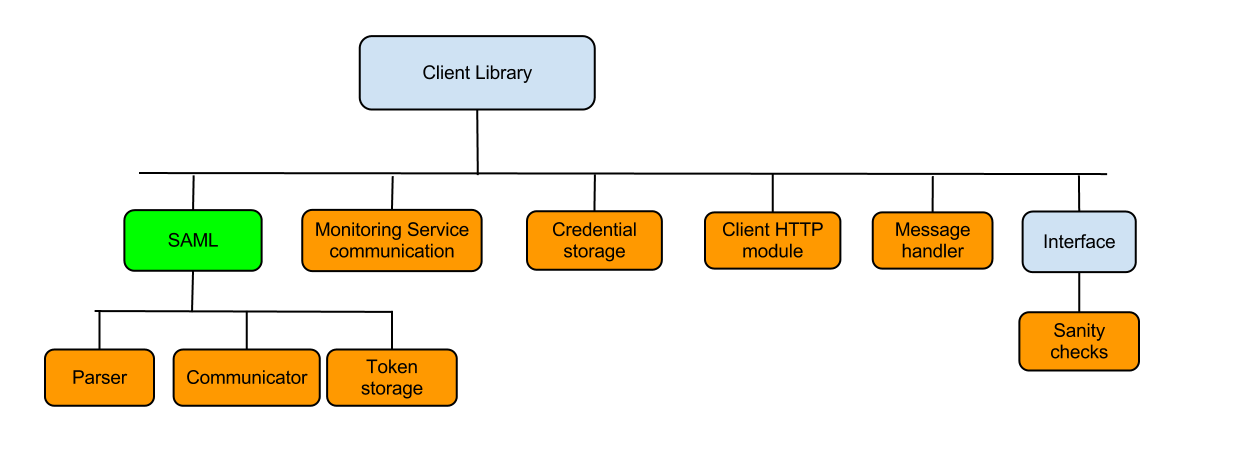
\includegraphics[width=\textwidth]{WorkbreakdownstructureClient}
            \caption{WBS-Client}
            The work break down structure for the client.
            \label{fig:WorkbreakdownstructureClient}
        \end{figure}
        
        \begin{figure}[H]
            \centering
            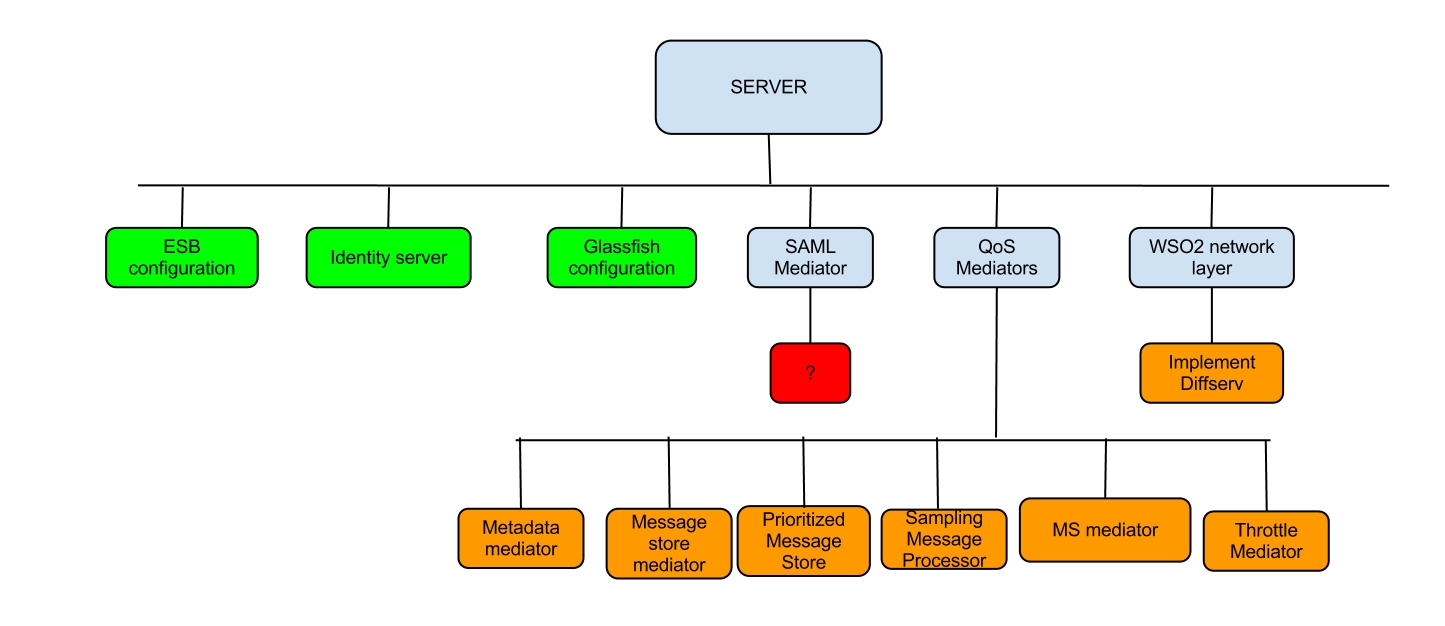
\includegraphics[width=\textwidth]{WorkbreakdownstructureServer}
            \caption{WBS-Server}
            The work break down structure for the server.
            \label{fig:WorkbreakdownstructureServer}
        \end{figure}

\section{File Attachments}\label{File Attachments} 
The files can be unpacked using the pdftk program in Linux with the command: 
    pdftk filetest.pdf unpack\_files \\
    \attachfile[description=Risk List,icon=Paperclip]{graphics/risklist.pdf} Risk List \\
    \attachfile[description=gantt,icon=Paperclip]{graphics/gantt.html} Gantt Diagram \\
    \attachfile[description=Introduction to the assignment,icon=Paperclip]{graphics/bachelor-QoS.pdf} Quality of Service (QoS) support for Web services in military networks \\
    
%    \attachfile[description=TEST log,icon=Paperclip]{report.log} Paperclip
%    \attachfile[description=TEST log,icon=Graph]{report.log} Graph
%    \attachfile[description=TEST log,icon=PushPin]{report.log} PushPin
%    \attachfile[description=TEST log,icon=Tag]{report.log} Tag

\begin{thebibliography}{0}
%  \begin{Bib - template}
%       \bibitem{Dumy00} Dummy Dum,
%           \emph{\LaTeX: A Dummy Bibliography Item}.
%           Latex Experts, Lake Tahoe,
%           4nd Edition,
%           ca 1000.
%   \end{Bib - template}

    %must be corrected.
    \bibitem{soa-qos-pdf} Dummy Dum, 
        \emph{\LaTeX: soa-qos-pdf}.
        Latex Experts, Lake Tahoe,
        4nd Edition,
        ca 1000.

\end{thebibliography}



\end{document}
